\documentclass[12pt]{report}
\usepackage[margin=1in]{geometry}
\usepackage{multicol}
\usepackage{caption}
\usepackage{subcaption}
\usepackage{graphicx}
\usepackage{float}
\usepackage{epstopdf}
\usepackage{setspace}
\usepackage{abstract}
%\usepackage{grffile}
\usepackage{pdfpages}
\usepackage{lscape}
\usepackage{authblk}
\usepackage{hyperref}

%Graphics Path
\graphicspath{{./MCINTOSH_Images/}{./WILEY_Images/}{./KIRBY_Images/}{./WESLEY_Images/}{./IANNUCCI_Images/}{./BLUM_Images/}{./REGAN_Images/}}

\usepackage{fancyhdr}
	\pagestyle{fancy}
	\fancyhead[L]{\today}
	\fancyfoot{}
	\fancyhead[C]{OCE 496 Section 2}
	\fancyhead[R]{\thepage}


\title{\vspace{-5mm}
	\fontsize{20pt}{10pt}\selectfont
	Embedded Wireless Sensor Design for Long Term Structural Health Monitoring
}
		
\author[2]{Christopher Bessin}	
\author[1]{Patrick Blum}
\author[1]{Matthew P. Iannucci}
\author[1]{Jordan T. Kirby}
\author[1]{Zachary McIntosh}
\author[2]{Elizabeth L. Paul}
\author[1]{Michael A. Regan}
\author[2]{Justin W. Skenyon}
\author[1]{Charles J. Wesley}
\author[1]{Samuel D. Wiley}

\affil[1]{Finite Element Modelling}
\affil[2]{Instrumentation Development}
\date{\normalsize\vspace{-3mm}\today}



\begin{document}
\maketitle

%Signature Block

\textit{I have read this paper in its entirety and approve it for submission.}
\vspace{1.5cm}

\noindent\begin{tabular}{ll}
\makebox[2.5in]{\hrulefill} & \makebox[2.5in]{\hrulefill}\\
Christopher Bessin & Date\\[4ex]% adds space between the two sets of signatures
\makebox[2.5in]{\hrulefill} & \makebox[2.5in]{\hrulefill}\\
Patrick Blum & Date\\[4ex]
\makebox[2.5in]{\hrulefill} & \makebox[2.5in]{\hrulefill}\\
Matthew P. Iannucci & Date\\[4ex]
\makebox[2.5in]{\hrulefill} & \makebox[2.5in]{\hrulefill}\\
Jordan T. Kirby & Date\\[4ex]
\makebox[2.5in]{\hrulefill} & \makebox[2.5in]{\hrulefill}\\
Zachary McIntosh & Date\\[4ex]
\makebox[2.5in]{\hrulefill} & \makebox[2.5in]{\hrulefill}\\
Elizabeth L. Paul & Date\\[4ex]
\makebox[2.5in]{\hrulefill} & \makebox[2.5in]{\hrulefill}\\
Michael A. Regan & Date\\[4ex]
\makebox[2.5in]{\hrulefill} & \makebox[2.5in]{\hrulefill}\\
Justin W. Skenyon & Date\\[4ex]
\makebox[2.5in]{\hrulefill} & \makebox[2.5in]{\hrulefill}\\
Charles J. Wesley & Date\\[4ex]
\makebox[2.5in]{\hrulefill} & \makebox[2.5in]{\hrulefill}\\
Samuel D. Wiley & Date\\[4ex]
\end{tabular}

%Abstract Here
Structural Health monitoring is the process of evaluating and assessing fatigue of existing infrastructure by continuously monitoring a long term change in
natural frequency vibration.
Aging traffic infrastructure is a growing problem across the world as material and construction cost has risen considerably in
recent decades.
As replacement becomes more difficult reliable lifetime extension is possible through structural health monitoring.
At the completion of this project a sensor package was designed and partially assembled, a simple finite element model (FEM) of the main span was produces, high precision
GPS units were installed and collected data for two weeks, and preliminary data was collected with the package accelerometers on top of the towers of
the bridge.
With development and research damage location, type, and severity may be indicated by interpreting the vibration changes. 



\tableofcontents
\listoffigures
\listoftables

\chapter{Introduction}
\label{ch:Paper_Introduction}
	\section{Objectives}
		\subsection{Phase One}
		\subsection{Phase Two}
	\section{Layout}
		\chapter{Finite Element Model (FEM)}

\section{Introduction}

\label{sec:examples}

\subsection{Background of the Claiborne Pell Bridge}

The Pell Bridge is 10,3471 in total length and has a main span on 1,601 feet making it the 83rd largest suspension bridge in the world. Traffic from
Aquidneck Island would otherwise have to drive around the bay through Providence if the Newport Bridge did not exist. The original proposal for the
bridge was submitted in 1950 by the designer of the New York City subway system and the Cape Cod Canal, and was approved in 1965. The concrete footings
the support the two towers are supported by 838 driven steel piles. At a water depth of 162 feet the foundation created for the Newport Bridge
involved the deepest pile driving in the world at this time. To accelerate cutting the tops of the piles, a dive tank was sunk that housed the divers
for a weeks at a time. Barges brought prefabricated sections of the bridge to Newport where they were lifted into place; the largest of the sections
weighted more than 400 tons and stood 10 stories high. 90,000 cubic yards of concrete were poured into the 52 piers \cite{RIBTA}\\ 

\subsection{Introduction to FEM}

A finite element model analyzes the physical response of a system to dynamic or static loading. The system is divided into finite elements and material
structural properties are applied. The physical response of the structure to an applied loading is added to the initial configuration of the structure.
Abaqus is a computer software which calculates approximate non linear finite element solutions for displacements, deformation, stresses, forces, etc. .
The state of the model is updated throughout the analysis steps and the effects of the previous step are included in the solution to each iteration
\cite{Abaqus}. The stiffness matrix and friction between elements are considered in its original state and updated after each iteration. \cite{Manoj}\\

\indent To verify the software the analysis of a simple system can be completed analytically and compared with the results of the program. For a simply
supported beams the modal shapes are trivial, however, the modal response for a complex structure, like the Claiborne Pell Bridge, anticipating modal
response is near impossible with analytical solutions. \\
\indent Abaqus provides multiple ways to model a particular structure. When modeling the Newport Bridge it will be necessary to use the physical
properties, such as length and profile, rather than physical properties, such as moment of inertia, to model efficiently. To ensure that Abaqus is
calculating moment of inertia as anticipated, analytical solutions can be compared with the results modal frequencies of the Abaqus model. Abaqus allows
for two different options of modeling, inputting the moment of inertia or imputing the profile of the element and allowing Abaqus to calculate moment
of inertia. \\
\indent Within a model produced in Abaqus, the removal of members allows for the structural integrity of the structure to be evaluated as an incomplete
system. Future construction can be aided by this as the ability to see if a partial structure can support itself. The loss of structural components can
be evaluated if lost as well. If a tower were to be damages by a boat or a hanger were to fail, the repercussion could be evaluated. 

\section{Abaqus FEM Verification}

\subsection{L Beam Analysis}

As Abaqus is solving Euler-Bernoulli beam theory equations and iterating the solution over a system, if the system is simple the analytical solution can be
found by hand. For the modal analysis of the 6.8 meter L beam, the beam was modeled two different ways in Abaqus. This was done to confirm that Abaqus
calculates the mode shapes and associated frequencies properly. The analytical solution was calculated using this Equation:


\ref{eqn:FEM_Anal}\\

\begin{equation}

F_{n}=\frac{1}{2\pi}\biggl[\frac{n \pi}{L} \biggr]^{2}\sqrt{[\frac{EI}{\rho}} , n=1,2,3\dots\infty

\label{eqn:FEM_Anal}

\end{equation}

\noindent The inputs for the analytical calculations and the Abaqus model are displayed in Table (Table 

\ref{tab:FEM_Abaqus_Comp}):\\

\indent The beam was modeled in Abaqus as 6.8 meters long, with the supports 0.35 meters from either end. There is a tri-axial restriction boundary
condition at one end and a vertical restriction boundary condition at the other. For the initial model, an undefined profile was used and the moment of
inertia and cross sectional area were input. In the second model, a preset profile was used and Abaqus calculated the moment of inertia. Thickness and
outer dimension of the beam were input. A comparison of the results of those models are presented in comparison to the analytical calculation as
follows:

(Table \ref{tab:FEM_Abaqus_Comp}):\\

\begin{table}[H]

\begin{center}

\begin{tabular}{|l| p{3.5cm}| p{3cm}| p{3cm}| p{3cm}|}

\hline

\textbf{Mode} & \textbf{Analytical Values} & \textbf{General Profile Abaqus Model Frequency}& 

\textbf{Input Profile Abaqus Model Frequency} \\\hline

1 & 3.1 Hz & 3.1 Hz & 3.1 Hz \\\hline

2 & 12.4 Hz & 12.5 Hz & 12.4 Hz \\\hline

3 & 27.9 Hz & 27.8 Hz & 27.8 Hz \\\hline

4 & 49.6 Hz & 48.8 Hz & 48.6 Hz \\\hline

5 & 77.5 Hz & 74.5 Hz & 74.4 Hz \\\hline

\end{tabular}

\caption{\textit{Comparison between Abaqus models}}

\label{tab:FEM_Abaqus_Comp}

\end{center}

\end{table}

\indent The frequencies of the analytical solution and the Abaqus model are very close. This is very important to the progression of this project as
Abaqus must be trusted to calculate the moment of inertia within the program, translating to correct modal shapes and frequencies. \\
\indent Analysis of an I beam was done as preliminary model verification and can be found in the Appendix ******. Because the corresponding frequencies
for the first 5 modes are more than three orders of magnitude larger than that is expected of the Claiborne Bridge (0.155-0.993Hz vs 17.6-230.1Hz), and
intentions for the beam were to test accelerometer setups to be used on the bridge, analysis was not continued on the I-beam and the L-beam was
introduced. 

\section{Claiborne Pell Bridge Model}

\subsection{Modeling Large Suspension Bridges}
The complexity and variability of large suspension bridges makes both numerical and experimental methodology very difficult and requires many assumptions.
As material and construction technologies advance, so do the length and structural complexity of these structures grow. Monitoring and measuring the
structural integrity of these bridges is very important as fatigue is very difficult to measure and quantify. Of the failure endured by steel
structures, 80-90\% are related to fatigue \cite{Chan}. Fatigue analysis includes evaluating the distribution of stress in structures.\\
\indent Long suspension bridges are very flexible and lightly damped structures that are largely impacted by the dynamic loading of cars, wind, and
environmental factors. Fatigue damage will result in large infrastructure due long-term cyclic loading in a corrosive environment
\cite{Chan,Guo,Li:2003}. As with many bridges that experience extreme season change, the Claiborne Pell Bridge is subject to varying temperature change,
snow loading, and salting in addition to the range of other challenges. 


\subsection{Modeling Process}

The purpose of the analysis of the model in Abaqus is to understand the bridge behavior during static loading. As the physical properties of the bridge
structural elements must be reflected in the model, the method of translating the blueprint in ABAQUS properly is vital to producing accurate results.
The main span of the Claiborne Pell Bridge was modeled in MKS (meter, kilogram, second) units. Each of the 8,233 elements were given the appropriate
dimension and material properties to reflect the beams and cables the Claiborne Pell Bridge. There are five structural components of a suspension
bridge 

which will be discussed in detail:

\begin{enumerate}
\item Main cables
\item Towers that support the cable system
\item Hanger cables
\item Anchor bolts that support the cable system at the ends of the cable
\item Hanger cables that connect the main cable to the deck
\item Girder
\end{enumerate}

\subsubsection{Main Cables and Hanger Cables}

Suspension bridges are the lightest bridges per foot made possible because by the weight bearing abilities of the cables which are made of thousands of
pencil-thin steel wires. Steel that is stretched into wires can withstand more stress. The tension force applied to the bridge girder are transferred to
the main cables through the hangers. The cables are very still and flex very little but need to allow for dynamic loading and vibrations \cite{manoj}.
The hanger and main cables are very complicated to model as they must be modeled with the anticipation that after loaded they will accurately represent
the physical shape and rigidity of the actual cables. It is now routine to measure the actual initial stresses in the hangers and main cables upon
construction to input into Abaqus for Eigenvalue analysis. As initial stress in the hangers and main cable will significantly affect the structural
stiffness matrix, K, it is imperative that this value be accurate. The Eigen values were calculated as follows: 

% FIX EQUATION 

\begin{equation}

( 2 \mu[M] + \mu[C] + [K]){\Phi} = 0

\label{eqn:Euler}

\end{equation}

Where [M] is the mass matrix, [C] is the damping matrix, and [K] is the stress matrix, $\mu$ is the 

eigenvalue, and $\Phi$ is the eigenvector \cite{manoj}. 

\subsubsection{Towers}

Made of steel, the towers are subjected to compressive forces induced by the main cables. They need to be sturdy enough to resist buckling, oscillations,
and flexing. The materials of towers is typically steel but in appropriate environments, concrete enforced steel is chosen. The current speed, price,
appearance, and whether salt water or fresh water is being gaped will depict what material is chosen \cite{manoj}. 


\subsubsection{Anchor Bolts}

Anchor piers bear the weight of the main cables and fix them in place. The anchor piers for the Claiborne Pell Bridge are 40x50x100 feet above the MWL and
weigh approximately 3,950 tons each. The weight of the anchor piers hold the cables in place. 

\subsubsection{Girder}

The function of the girder is to stiffen the roadway and support the road deck which carries traffic. The girder is very stiff and thus inhibits large
variations in the road deck as concentrated loads travel over the bridge.\\ 
\indent It was the unfavorable trapezoidal shape of the girder that lead to the collapse of the Tacoma Bridge. The span to width ratio and shape allowed
wind excite the bridge dramatically. After the collapse of the Tacoma Bridge the girder shapes were made to be more stiff with diagonal supports and
square rather than sharp edged \cite{}. 

\subsection{Limitations of Abaqus Model}

\indent Although finite element analysis has enables engineers and scientists gain an understanding of a structure's behavior and dynamic response, it is
very important to know the limitations of finite element modeling. Abaqus must be used as a research tool and not considered the basis of design
\cite{Abaqus}. When verifying experimental data, a FEM should not be used for analysis as too many variables that can not be measured or controlled. \\
\indent In phase one of this project and indicating a particular profile, the preset profiles that are available do not match identically with the
profiles that were used in experiments. The taper of the flange and the radius of the angle were not taken into account in the profile provided by
Abaqus. As the frequencies resultant for the two different modeling techniques were not considerably different, the error acquired within the
dissimilarity is assumed not to be significant and thus neglected in evaluations. \\
\indent In phase two of this project, many assumptions and simplifications were made to allow for preliminary modeling. The method of modeling for this
semester does not consider mated elements; the entire structure is considered as one highly elastic structure with varying physical properties rather
than many different pieced welded or joined with bolts. This affects how the bridge moves as no friction between parts and no welds are considered. 
\indent Fatigue damage is local failure mode and occurs most often in welded regions and thus the model should include the detailed welded region
connection points. The stress fluctuations are very low so the structure will deform elastically except in the welded regions. Critical locations for
fatigue damage can be identified by global stress estimation. As the properties of the bridge elements \cite{manoj}\\
		
\chapter{Finite Element Model (FEM)}
\label{ch:FEM}
	%\chapter{Finite Element Model (FEM)}

\section{Introduction}

\label{sec:examples}

\subsection{Background of the Claiborne Pell Bridge}

The Pell Bridge is 10,3471 in total length and has a main span on 1,601 feet making it the 83rd largest suspension bridge in the world. Traffic from
Aquidneck Island would otherwise have to drive around the bay through Providence if the Newport Bridge did not exist. The original proposal for the
bridge was submitted in 1950 by the designer of the New York City subway system and the Cape Cod Canal, and was approved in 1965. The concrete footings
the support the two towers are supported by 838 driven steel piles. At a water depth of 162 feet the foundation created for the Newport Bridge
involved the deepest pile driving in the world at this time. To accelerate cutting the tops of the piles, a dive tank was sunk that housed the divers
for a weeks at a time. Barges brought prefabricated sections of the bridge to Newport where they were lifted into place; the largest of the sections
weighted more than 400 tons and stood 10 stories high. 90,000 cubic yards of concrete were poured into the 52 piers \cite{RIBTA}\\ 

\subsection{Introduction to FEM}

A finite element model analyzes the physical response of a system to dynamic or static loading. The system is divided into finite elements and material
structural properties are applied. The physical response of the structure to an applied loading is added to the initial configuration of the structure.
Abaqus is a computer software which calculates approximate non linear finite element solutions for displacements, deformation, stresses, forces, etc. .
The state of the model is updated throughout the analysis steps and the effects of the previous step are included in the solution to each iteration
\cite{Abaqus}. The stiffness matrix and friction between elements are considered in its original state and updated after each iteration. \cite{Manoj}\\

\indent To verify the software the analysis of a simple system can be completed analytically and compared with the results of the program. For a simply
supported beams the modal shapes are trivial, however, the modal response for a complex structure, like the Claiborne Pell Bridge, anticipating modal
response is near impossible with analytical solutions. \\
\indent Abaqus provides multiple ways to model a particular structure. When modeling the Newport Bridge it will be necessary to use the physical
properties, such as length and profile, rather than physical properties, such as moment of inertia, to model efficiently. To ensure that Abaqus is
calculating moment of inertia as anticipated, analytical solutions can be compared with the results modal frequencies of the Abaqus model. Abaqus allows
for two different options of modeling, inputting the moment of inertia or imputing the profile of the element and allowing Abaqus to calculate moment
of inertia. \\
\indent Within a model produced in Abaqus, the removal of members allows for the structural integrity of the structure to be evaluated as an incomplete
system. Future construction can be aided by this as the ability to see if a partial structure can support itself. The loss of structural components can
be evaluated if lost as well. If a tower were to be damages by a boat or a hanger were to fail, the repercussion could be evaluated. 

\section{Abaqus FEM Verification}

\subsection{L Beam Analysis}

As Abaqus is solving Euler-Bernoulli beam theory equations and iterating the solution over a system, if the system is simple the analytical solution can be
found by hand. For the modal analysis of the 6.8 meter L beam, the beam was modeled two different ways in Abaqus. This was done to confirm that Abaqus
calculates the mode shapes and associated frequencies properly.
The analytical solution was calculated using Equation \ref{eqn:FEM_Anal}.
The inputs for the analytical calculations and the Abaqus model are displayed in Table \ref{tab:FEM_Abaqus_Comp}

\begin{equation}
F_{n} = \frac{1}{2\pi} \biggl[ \frac{n \pi}{L} \biggr ]^{2} \sqrt{\frac{EI}{\rho}}, n=1,2,3 \dots \infty
\label{eqn:FEM_Anal}
\end{equation}

\indent The beam was modeled in Abaqus as 6.8 meters long, with the supports 0.35 meters from either end. There is a tri-axial restriction boundary
condition at one end and a vertical restriction boundary condition at the other. For the initial model, an undefined profile was used and the moment of
inertia and cross sectional area were input. In the second model, a preset profile was used and Abaqus calculated the moment of inertia. Thickness and
outer dimension of the beam were input. A comparison of the results of those models are presented in comparison to the analytical calculation as
follows:

%(Table \ref{tab:FEM_Abaqus_Comp}):\\ 		%Unnecessary?

\begin{table}[H]

\begin{center}

\begin{tabular}{|l| p{4cm}| p{4cm}| p{4.5cm}| p{4.5cm}|}

\hline

Mode & Analytical Values & General Profile Abaqus Model Frequency&  Input Profile Abaqus Model Frequency \\

\hline

1 & 3.1 Hz & 3.1 Hz & 3.1 Hz \\\hline

2 & 12.4 Hz & 12.5 Hz & 12.4 Hz \\\hline

3 & 27.9 Hz & 27.8 Hz & 27.8 Hz \\\hline

4 & 49.6 Hz & 48.8 Hz & 48.6 Hz \\\hline

5 & 77.5 Hz & 74.5 Hz & 74.4 Hz \\\hline

\end{tabular}

\caption{\textit{Comparison between Abaqus models}}

\label{tab:FEM_Abaqus_Comp}

\end{center}

\end{table}

\indent The frequencies of the analytical solution and the Abaqus model are very close. This is very important to the progression of this project as
Abaqus must be trusted to calculate the moment of inertia within the program, translating to correct modal shapes and frequencies. \\
\indent Analysis of an I beam was done as preliminary model verification and can be found in the \textbf{\textit{Appendix}} ******. Because the corresponding frequencies
for the first 5 modes are more than three orders of magnitude larger than that is expected of the Claiborne Bridge (0.155-0.993Hz vs 17.6-230.1Hz), and
intentions for the beam were to test accelerometer setups to be used on the bridge, analysis was not continued on the I-beam and the L-beam was
introduced. 

\section{Claiborne Pell Bridge Model}

\subsection{Modeling Large Suspension Bridges}
The complexity and variability of large suspension bridges makes both numerical and experimental methodology very difficult and requires many assumptions.
As material and construction technologies advance, so do the length and structural complexity of these structures grow. Monitoring and measuring the
structural integrity of these bridges is very important as fatigue is very difficult to measure and quantify. Of the failure endured by steel
structures, 80-90\% are related to fatigue \cite{Chan}. Fatigue analysis includes evaluating the distribution of stress in structures.\\
\indent Long suspension bridges are very flexible and lightly damped structures that are largely impacted by the dynamic loading of cars, wind, and
environmental factors. Fatigue damage will result in large infrastructure due long-term cyclic loading in a corrosive environment
\cite{Chan}. As with many bridges that experience extreme season change, the Claiborne Pell Bridge is subject to varying temperature change,
snow loading, and salting in addition to the range of other challenges. 


\subsection{Modeling Process}

The purpose of the analysis of the model in Abaqus is to understand the bridge behavior during static loading.
As the physical properties of the bridge
structural elements must be reflected in the model, the method of translating the blueprint in ABAQUS properly is vital to producing accurate results.
The main span of the Claiborne Pell Bridge was modeled in MKS (meter, kilogram, second) units.
Each of the 8,233 elements were given the appropriate
dimension and material properties to reflect the beams and cables the Claiborne Pell Bridge. 
There are five structural components of a suspension
bridge which will be discussed in detail:

\begin{enumerate}
\item Main cables
\item Towers that support the cable system
\item Hanger cables
\item Anchor bolts that support the cable system at the ends of the cable
\item Hanger cables that connect the main cable to the deck
\item Girder
\end{enumerate}

\subsubsection{Main Cables and Hanger Cables}

Suspension bridges are the lightest bridges per foot made possible because by the weight bearing abilities of the cables which are made of thousands of
pencil-thin steel wires. Steel that is stretched into wires can withstand more stress. The tension force applied to the bridge girder are transferred to
the main cables through the hangers. The cables are very still and flex very little but need to allow for dynamic loading and vibrations \cite{manoj}.
The hanger and main cables are very complicated to model as they must be modeled with the anticipation that after loaded they will accurately represent
the physical shape and rigidity of the actual cables. It is now routine to measure the actual initial stresses in the hangers and main cables upon
construction to input into Abaqus for Eigenvalue analysis. As initial stress in the hangers and main cable will significantly affect the structural
stiffness matrix, K, it is imperative that this value be accurate. The Eigenvalues were calculated as follows: 

% FIX EQUATION 

\begin{equation}
( 2 \mu [M] + \mu [C] + [K]) {\Phi} = 0
\label{eqn:Euler}
\end{equation}

Where [M] is the mass matrix, [C] is the damping matrix, and [K] is the stress matrix, $\mu$ is the 

eigenvalue, and $\Phi$ is the eigenvector \cite{manoj}. 

\subsubsection{Towers}

Made of steel, the towers are subjected to compressive forces induced by the main cables. They need to be sturdy enough to resist buckling, oscillations,
and flexing. The materials of towers is typically steel but in appropriate environments, concrete enforced steel is chosen. The current speed, price,
appearance, and whether salt water or fresh water is being gaped will depict what material is chosen \cite{manoj}. 


\subsubsection{Anchor Bolts}

Anchor piers bear the weight of the main cables and fix them in place. The anchor piers for the Claiborne Pell Bridge are 40x50x100 feet above the MWL and
weigh approximately 3,950 tons each. The weight of the anchor piers hold the cables in place. 

\subsubsection{Girder}

The function of the girder is to stiffen the roadway and support the road deck which carries traffic. The girder is very stiff and thus inhibits large
variations in the road deck as concentrated loads travel over the bridge.\\ 
\indent It was the unfavorable trapezoidal shape of the girder that lead to the collapse of the Tacoma Bridge. The span to width ratio and shape allowed
wind excite the bridge dramatically. After the collapse of the Tacoma Bridge the girder shapes were made to be more stiff with diagonal supports and
square rather than sharp edged \cite{manoj}. 

\subsubsection{Modeling Technique}

The suspended portion of the Newport Bridge was modeled in three dimensions with an Abaqus input file. 
The model is made up of nodes and elements. The nodes are coordinates that define the location of the connection points of each element. 
The elements represent beams or beam segments. In total, 3198 nodes and 8233 elements were used to model the suspended portion of the bridge. 
This incudes the towers from the concrete base to the top of the towers vertically, and the cables, roadway and truss as far as the roadway is suspended. 
The cables at either end of the suspended portion and the base of the towers are modeled as fixed in all axes of translation and rotation (encaster).
The towers are made up of 50 nodes and 62 elements to describe the various sections and connection points. 
The links and pins connecting towers to the girder (truss under the roadway) consist of 14 nodes and 22 elements. 
The main cables were modeled using a second order polynomial fit for the center span and a fourth order polynomial fit for the side span. 
The lower portion of the hanger cables and roadway are described by a second order polynomial fit in the center span and a constant 4.6 \% grade outer span. 
The cables consist of 148 nodes for the main cables and upper connection points of the hanger cables.
The lower connection points of the hanger cables are connected to nodes along the truss. The main cables consist of 152 elements 


\subsection{Limitations of Abaqus Model}

\indent Although finite element analysis has enables engineers and scientists gain an understanding of a structure's behavior and dynamic response, it is
very important to know the limitations of finite element modeling. Abaqus must be used as a research tool and not considered the basis of design
\cite{Abaqus}. When verifying experimental data, a FEM should not be used for analysis as too many variables that can not be measured or controlled. \\
\indent In phase one of this project and indicating a particular profile, the preset profiles that are available do not match identically with the
profiles that were used in experiments. The taper of the flange and the radius of the angle were not taken into account in the profile provided by
Abaqus. As the frequencies resultant for the two different modeling techniques were not considerably different, the error acquired within the
dissimilarity is assumed not to be significant and thus neglected in evaluations. \\
\indent In phase two of this project, many assumptions and simplifications were made to allow for preliminary modeling. The method of modeling for this
semester does not consider mated elements; the entire structure is considered as one highly elastic structure with varying physical properties rather
than many different pieced welded or joined with bolts. This affects how the bridge moves as no friction between parts and no welds are considered. 
\indent Fatigue damage is local failure mode and occurs most often in welded regions and thus the model should include the detailed welded region
connection points. The stress fluctuations are very low so the structure will deform elastically except in the welded regions. Critical locations for
fatigue damage can be identified by global stress estimation. As the properties of the bridge elements \cite{manoj}\\


\chapter{Instrumentation Package}
\label{ch:Instrumentation}
	\section{Introduction}
	\section{Microprocessor}
		\subsection{Necessary Specifications}
		\subsection{Platform Options}
		\subsection{Final Platform}
	\section{Sensors}
		\subsection{Accelerometer}
			\subsubsection{Necessary Specifications}
			\subsubsection{Sensor Options}
			\subsubsection{Sensor Selection}
		\subsection{Strain Gauge}
			\subsubsection{Necessary Specifications}
			\subsubsection{Sensor Options}
			\subsubsection{Sensor Selection}
		\subsection{GPS Receiver}
			\subsection{Global Positioning System (GPS) Receiver}
\indent The need for an accurately synchronized timing system was present throughout the planning of the sensor package in order to synchronize data from
multiple sensor packages. The internal clock on the microprocessor board was determined to be unreliable due to inherent errors from low tolerances in CPU
clock crystals. The use of a GPS receiver as an external timing source was explored \cite{GPSTimeSync}.
\subsection{GPS Parameters}
\label{sec:GPS_Parameters}
\indent The following parameters were considered when choosing the GPS receiver for time-synchronization:
\begin{itemize}
\item Power Consumption 
\item Pulse Per Second (PPS) Output Signal
\item Communicate via Serial Interface
\end{itemize}
\paragraph{Power Consumption}
\label{sec:GPS_power_cons.}
\indent As for all other components in the sensor package, the GPS needed to have a low power draw. The GPS receiver was anticipated as being the sensor
with the highest power consumption.
%
\paragraph{Pulse Per Second (PPS) Output Signal}
\label{sec:gps_out_ch_num}
\indent It is proposed for future use that the PPS signal be used for time synchronizing the data between multiple sensor packages.

\paragraph{Communication}
\label{sec:adc_comm}
\indent Due to the communication protocols that the microprocessor supports, found in Section \ref{sec:uProcessor}, the GPS must support UART, SPI or
I$^{2}$C communications as inputs.

\subsection{Trimble Copernicus II}
\label{sec:GPS_Trimble}
\indent The Trimble Copernicus II (Figure \ref{fig:GPS_Copernicus}) is a 12-channel, PCB mounted GPS. The GPS features two serial ports and a 3.0v PPS
output signal, shown in Figure \ref{fig:GPS_PPS}. The power consumption of the package is approximately $132mW$ at $3V$. This receiver was chosen as a
prototyping solution because it was available in a dual in-line package (DIP), making it easily interfaced on a breadboard. 

\begin{figure}
\centering
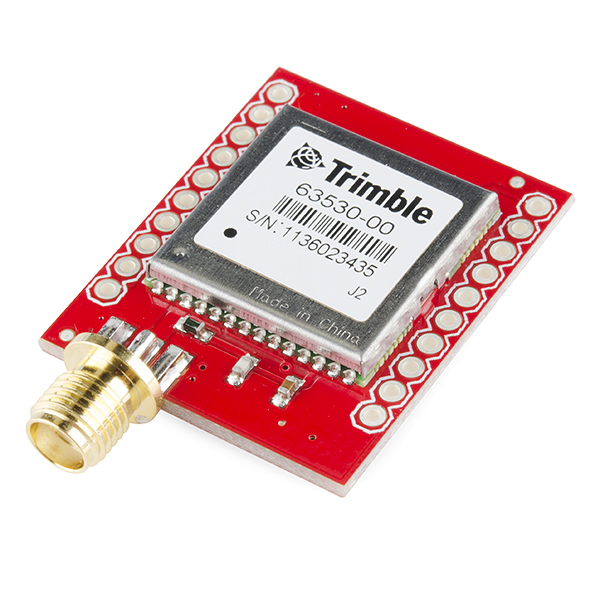
\includegraphics[width = 0.25\linewidth]{GPS_Copernicus}
\caption{\textit{Copernicus II GPS receiver}}
\label{fig:GPS_Copernicus}
\end{figure}

%\begin{landscape}
\begin{figure}[H]
\centering
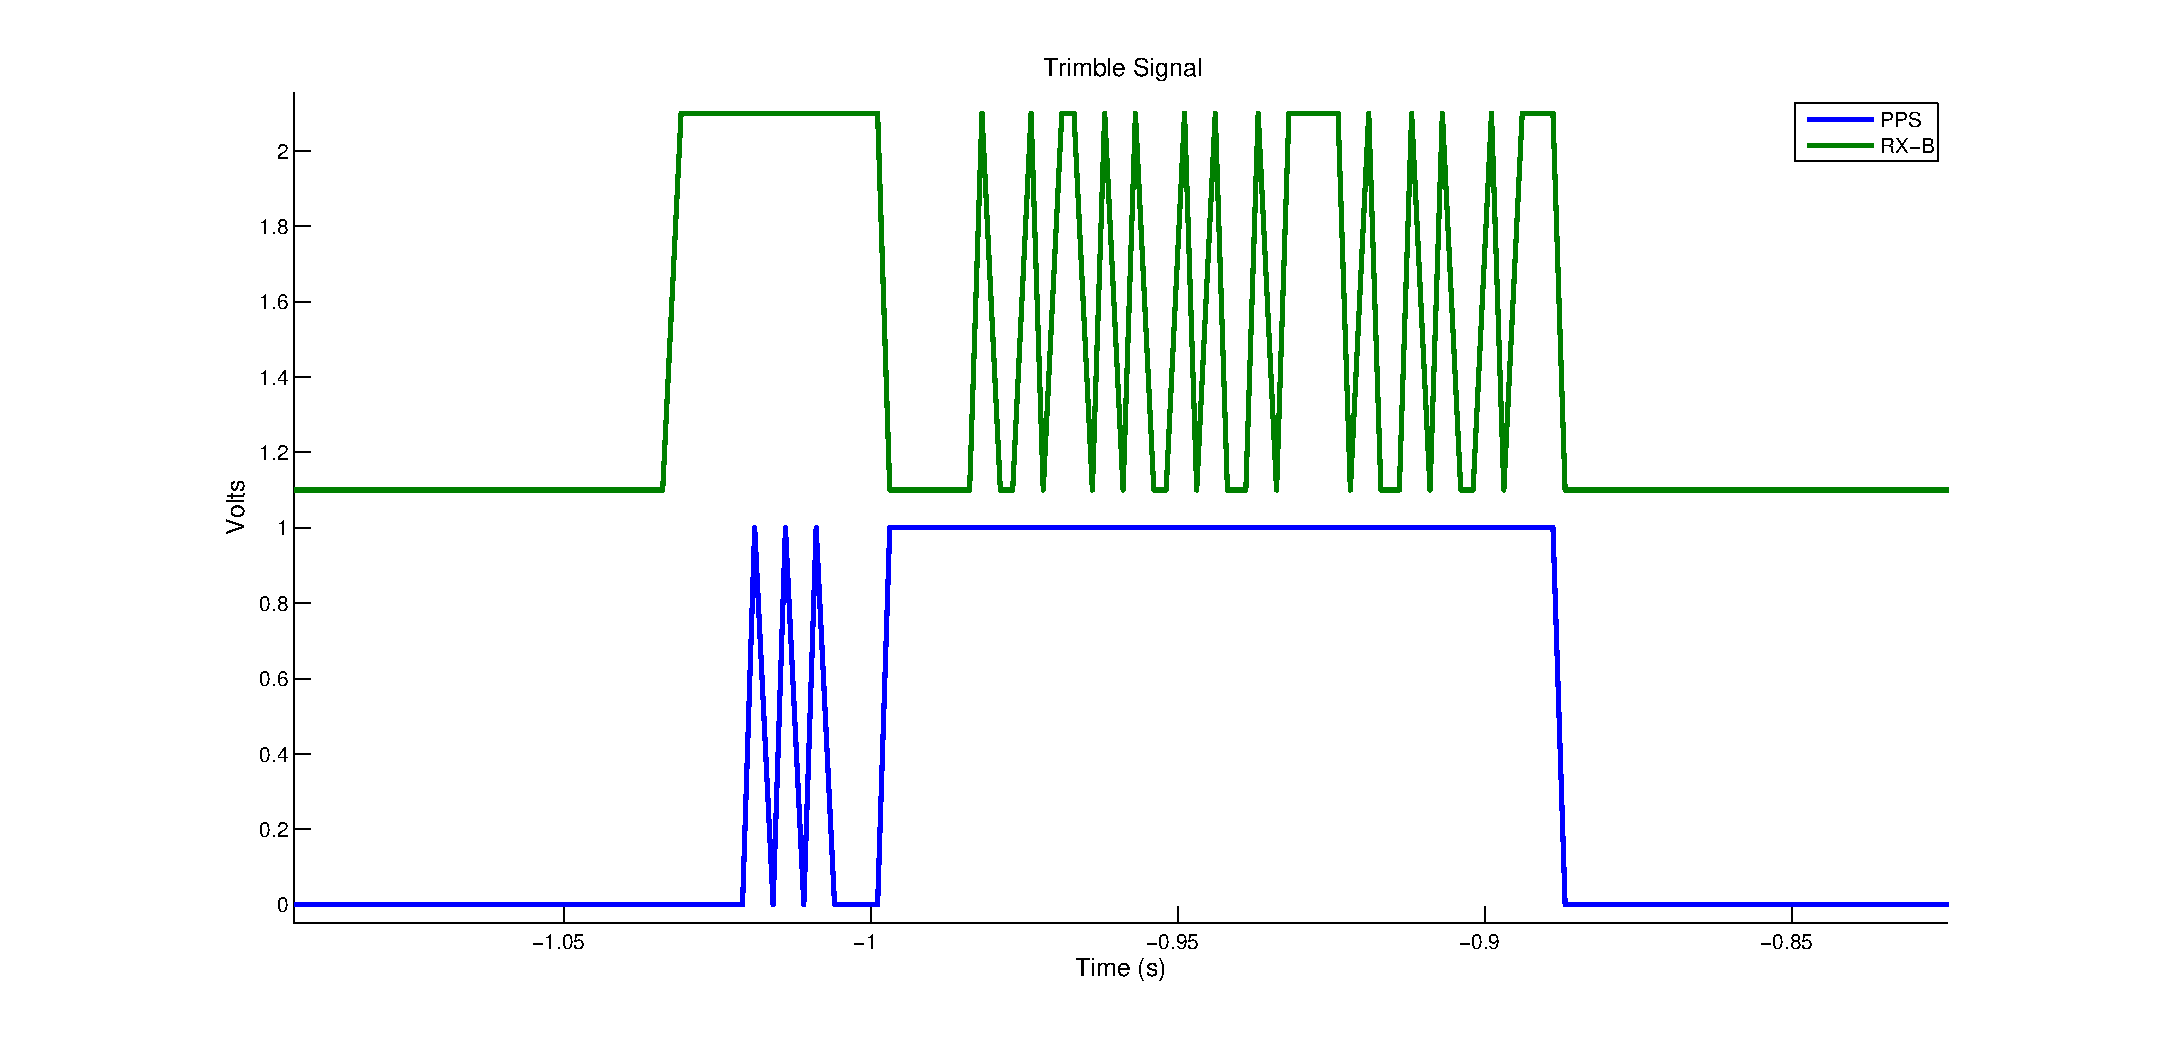
\includegraphics[width = 0.75\linewidth]{Trimble}
\caption{\textit{GPS sentence data and PPS signal recorded with oscilloscope for preliminary analysis.}}
\label{fig:GPS_PPS}
\end{figure}
%\end{landscape}
		\subsection{CORS}
		\subsection{Analog to Digital Converter}
			\section{Analog-to-Digital Data Converter}
\subsection{Necessary Specifications}
\label{sec:ADC_Parameters}
\indent The BeagleBone Black microcontroller features an on board 12-bit analog-to-digital converter (ADC). From literature, the lowest acceptable
effective resolution that an ADC being used for SHM may have is 16 bits\cite{Cunha_Caetano} \cite{JangSWMWSS}. It was determined that the need for an
external ADC was present. The parameters of the external ADC needed were as follows:
\begin{itemize}
\item High Resolution
\item Appropriate Sampling Frequency
\item Low Power Consumption 
\item Support for Multiple Input Channels
\item Communicate via Serial Interface
\end{itemize}
\subsubsection{Resolution}
\label{sec:adc_res}
\indent Resolution is defined as the number of bits that an analog signal is mapped to after being converted\cite{MusaJouaneh:2013}. Using the chart in
Figure \ref{fig:ADC_Comp_Chart}, it was evident that in order to achieve high resolution data that a Delta-Sigma ($\Delta\Sigma$) ADC needed to be used.\\
\indent As previously stated, the minimum resolution required for this sensor package was 16-bits. The voltage resolution can be found using Equation
\ref{eqn:Resolution}:
\begin{equation}
\label{eqn:Resolution}
V_{Res} = \frac{V_{Range}}{2^{n}}
\end{equation}
Assuming $V_{Range}=3.3V$, $n=16$ bits then $V_{Res}$ is approximately $50.35\mu V/$division. 

\begin{figure}[H]
\centering
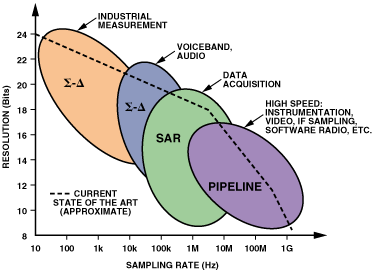
\includegraphics[scale=1]{./KIRBY_Images/ADC_Comp_Chart.jpg}
\caption{\textit{Chart displaying the classifications of different ADC architectures \cite{WaltKester:2005}}}
\label{fig:ADC_Comp_Chart}
\end{figure}
%
\subsubsection{Sampling Rate}		%EDIT THIS SECTION
\label{sec:adc_fin}
\indent The Nyquist-Shannon Sampling Criterion states that data must be sampled at a minimum of twice the expected frequencies being measured
\cite{MusaJouaneh:2013}. The accelerometer that was chosen for the preliminary lab experiments has a bandwidth of $500 Hz$, therefore the ADC must be able
to sample a minimum of $1kHz$. However, since frequencies expected from the lab testing are in the range of $0-60Hz$, the sampling frequency of the ADC
does not necessarily need to be so high. %Must reference source that states expected natural frequencies of bridges
%
\subsubsection{Power Consumption}
\label{sec:adc_power_cons.}
\indent Since the nature of this sensor package was to be a wireless sensor, it was assumed that all power used by the sensor package would be generated
using alternative energy. With this in mind, components used on board the sensor package have as little current draw as possible.
%
\subsubsection{Input Channels}
\label{sec:adc_in_ch_num}
\indent One important, but almost overlooked, characteristic of the ADC was the ability to support multiple input channels simultaneously. The ADC needed
to be able to read three channels from an accelerometer and at least two channels from a strain gauge. For prototyping purposes, it is typically difficult
to find ADC's with more than 4 inputs; most come in as surface mount components and require a printed circuit board. It became evident as the project progressed that each input device would need a dedicated ADC due to the multiplexer switching time of multi-channel ADC units. 
It was decided to address this problem by interfacing four ADC units simultaneously on a serial communication bus.
Subsection \ref{sec:adc_comm} discusses this in further detail.
It should also be noted that the inputs of the ADC were configured for differential measurements.
This gives the ability to compare the sensor data to a noise reference, and thus make reducing data filtering during processing. 
%
\subsubsection{Communication}
\label{sec:adc_comm}
\indent As shown in Table \ref{tab:uProcOptions}, the BeagleBone Black supports multiple communication protocols, include but not limited to, SPI and
I$^{2}$C. The communication from the ADC to the main micro-controller was decided to be either  4-wire SPI or I$^{2}$C. The ADC will be the slave to the
micro-controller. A con using SPI as the communication method is that for each slave device in the communication loop, there must be a dedicated Slave
Select (SS) line. This puts a limitation on how many ADC's can be used in each sensor package. However, I$^{2}$C utilizes a central bus and 7 bit unique
addresses for slave selection.

\subsection{Analog-to-Digital Converter Selection}
\indent When searching for ADC's that fit the parameters set in Section \ref{sec:ADC_Parameters}, three devices were investigated; the TI ADS1211, TI
ADS1115 and the TI ADS1113. The devices are summarized in Table \ref{tab:ADC_Compare} and explained in detail below.

\begin{table}[H]
\begin{center}
\begin{tabular}{|p{3cm}| p{3cm} | p{3cm} | p{3cm}|}
\hline
&\multicolumn{3}{c|}{\textbf{Analog-Digital Converter}}\\
\hline
\textbf{Parameter} & ADS1211 & ADS1115 & ADS1113\\
\hline
Package &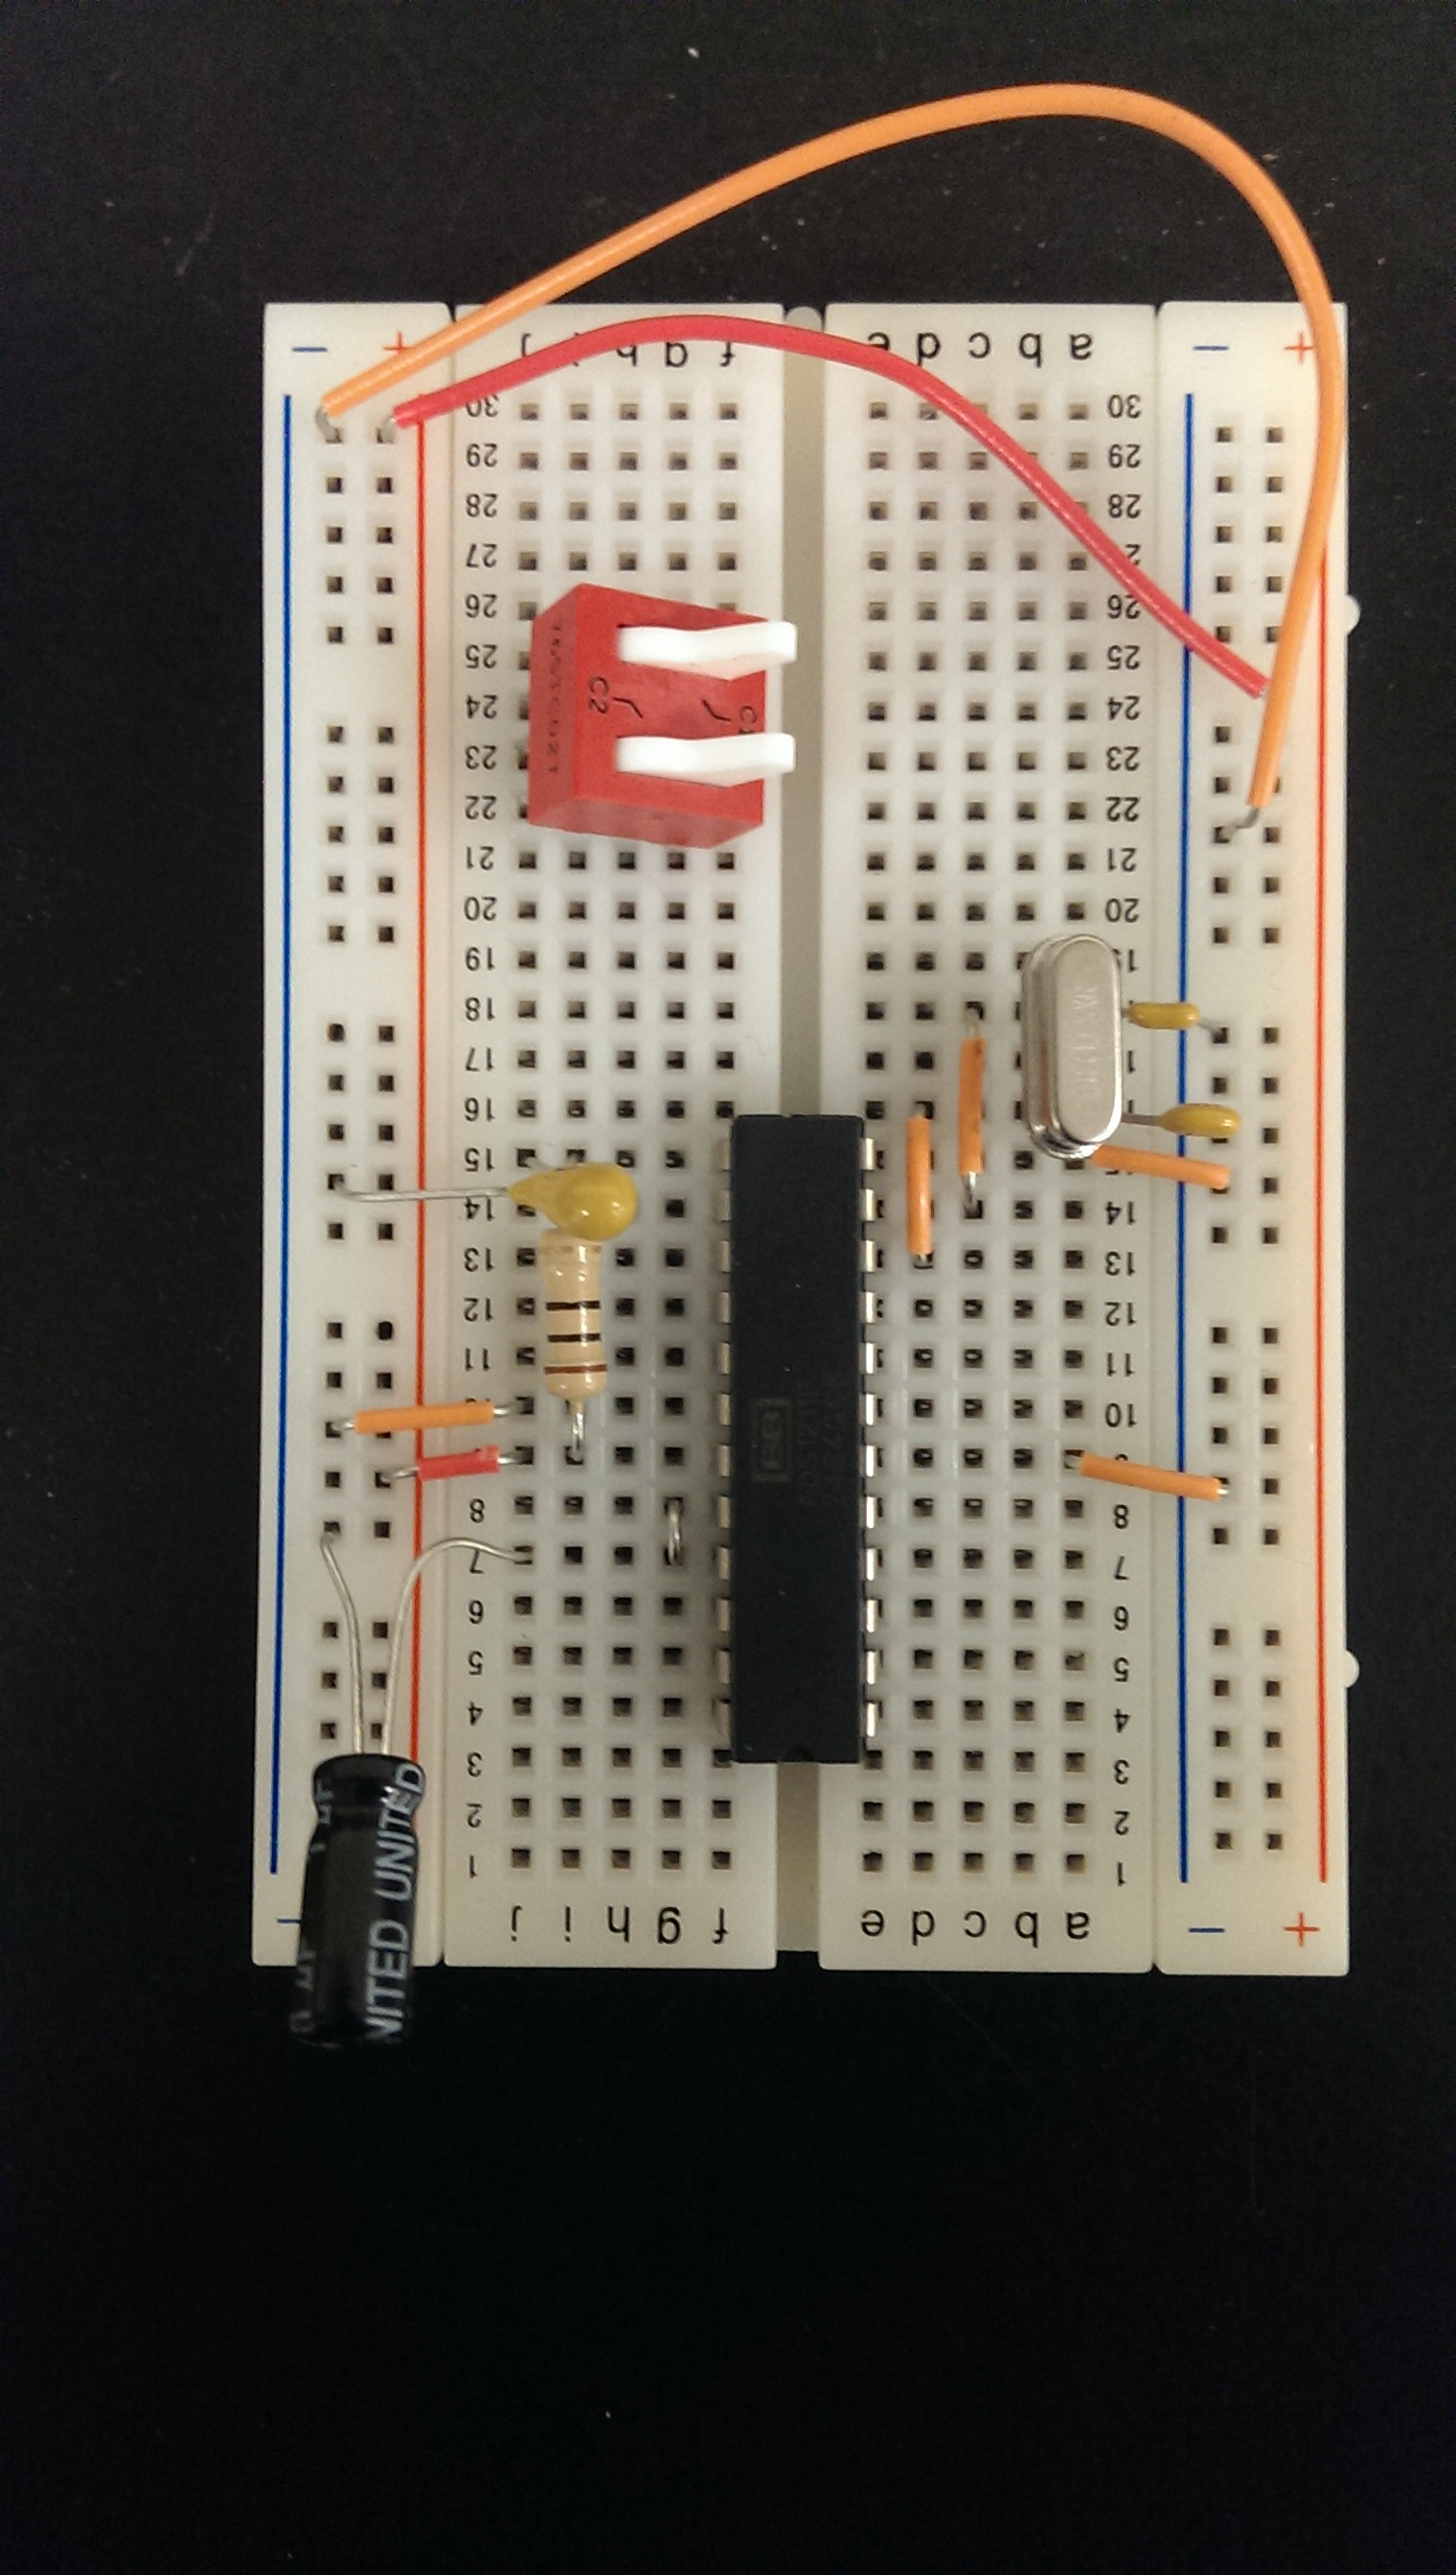
\includegraphics[width = 2.5cm]{./KIRBY_Images/oldadc}
&
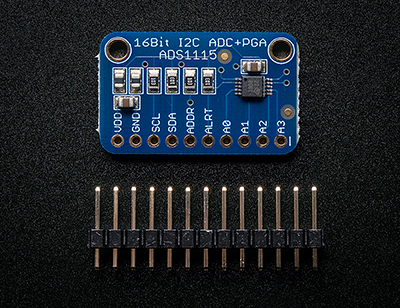
\includegraphics[width = 2.5cm]{./KIRBY_Images/ads1115} & 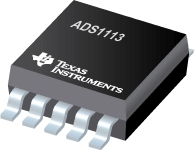
\includegraphics[width = 2.5cm]{./KIRBY_Images/ADS1113_msop10}\\
\hline
Resolution: & 24 bits & 16 bits & 16 bits\\
\hline
Supported Communications:&	 SPI & I$^2$C & I$^2$C \\
\hline
Power Consumption:&	5mW @ 5V	& 0.66 mW @ 3.3V & 0.66 mW @ 3.3V\\
\hline
Number of Inputs: & 4 & 4 & 1\\
\hline

\end{tabular}
\caption{\textit{Comparison table of the ADS1211, ADS1115 and ADS1113 ADC devices}}
\label{tab:ADC_Compare}
\end{center}
\end{table}


\subsubsection{TI ADS1211}
\label{sec:ADC_ADS1211}
\indent The Texas Instruments ADS1211 24-Bit $\Delta \Sigma$ analog to digital converter features 20 effective bits of resolution at $1kHz$ under ideal
conditions; however that would be contingent upon the ability to design an ideal printed ciruit board (PCB) for the converter. Between 16 and 18 bits of
resolution are realistic for the initial prototype of the sensor package. By utilizing an internal 4-to-1 multiplexer, four input channels are available
to use. Recall that Section \ref{sec:adc_in_ch_num} requires at least five input channels, the ADS1211 falls short here. As a solution two ADC's would
be used, making it possible to read two strain gauges per sensor package as opposed to one. The ADS1211 datasheet provides information on synchronizing
multiple ADC's together. The converter draws approximately $10mA$ under typical working conditions. The converter utilizes the SPI protocol that is
supported by the BeagleBone Black.\\
\indent The ADS1211 was purchased and interfaced; however due to the complex circuitry that was required by the device, a month passed before the chip was
tested. The converter functioned correctly for approximately ten minutes and then stopped transmitting data. 
\subsubsection{TI ADS1115}
\label{sec:ADC_ADS1115}
\indent The Texas Instruments ADS1115 16-Bit analog to digital converter is of the same architecture as the ADS1211 ($\Delta \Sigma$). The chip also
features a multiplexer that allows up to 4 single ended or 2 differential inputs. The sampling frequency of the ADC is programmable from 8Hz to 860Hz, and
includes an internal oscillator. The average current draw for the ADS1115 is approximately $150\mu A$. There are two notable differences between the
ADS1115 and the ADS1211 ADCs. First, the ADS1115 communicates via the I$^{2}$C communication protocol. The ADS1115 has four unique I$^{2}$C addresses;
making it possible to have 16 single-ended inputs on one communication bus. Also, the chip was available pre-mounted on a PCB with all the necessary
supporting hardware; thus eliminating the possibility of incorrectly wiring up the circuit. 
\subsubsection{TI ADS1113}
\label{sec:ADC_ADS1113}
\indent The TI ADS1113 is within the same family as the ADS1115, only differing in the number of input channels and not having internal programmable gain amplifiers and comparator.
Like the ADS1115, four ADS1113 units can be on the same I$^{2}$C bus, can also run in continuous sampling mode, and also shares the same library of functions as the ADS1115.
Since the ADS1113 does not multiplex its inputs, there is no loss of data between switching.
The dissadvantage to the ADS1113 is that it is only available as a surface mount chip (MSOP-10 package); thus requiring more circuitry on the printed circuit board.

\subsubsection{ADC Impedance Matching}
Preliminary lab tests were performed using a micro-controller with 12-bit ADC to collect data for analysis.
The time series that was returned did not accurately represent the data present, as verified with an oscilloscope.
It was determined that this was due to a difference in impedances between the accelerometer and the ADC.
The solution was to construct an op-amp circuit to match the impedances of the accelerometer and the micro-controller inputs.
It was initially believed that the internal programmable gain amplifiers (PGA) of the ADS1115 would avoid such issues in impedance matching.
However, after further research it was discovered that this assumption was incorrect.


\subsubsection{ADC Final Selection}
\indent Based on the comparison of the ADS1211, ADS1115 and ADS1113 ADC's, the ADS1115 was chosen for the preliminary package to test code before the printed circuit board was designed.
For the final package, four ADS1113 ADC units were integrated into the PCB design as discussed in Section \ref{sec:ADC_Impedance_Matching}. 

	\section{Electronics Design}
			\subsection{Introduction}
\indent The unique requirements for the sensor developed for deployment on the Claiborn Pell Newport Bridge set the sensor apart from off-the-shelf sensors readily available for purchase.
The sensor package needed to record high precision, high resolution accelerometer and strain gauge data continuously for an extended period of time. 
The longevity of the package was dependent upon the battery capacity and data storage capacity. 
This could have been solved by utilizing a large bank of batteries and multiple hard disk drives; however it was determined that this was a not a feasible option. 
Instead the sensor package would scavenge energy to recharge batteries and transmit data to a base station wirelessly. 
The addition of these two requirements greatly increased the complexity of the sensor package design. \\

\indent 

\subsection{Circuitry}

\subsubsection{Voltage Regulation}
The voltage input for most systems on the sensor board are a range of voltages between 3.3V-5V.
This posed a basic issue due to the output voltage of the 12V battery. 
The solution was to use two LM317 linear voltage regulators.
It was initially proposed to use the two regulators in series, such that the voltage dropped from 12V to 5V and then to 3.3V.
However, due to the current rating on the devices, it was decided to use the regulators in parallel and drop the voltage from 12V to 5V and 12V to 3.3V.
The complete circuit may be found in Figure \ref{fig:Schematic_VoltageReg}.
The LM317 technical specifications are displayed in Table \ref{tab:LM317} 

\begin{table}[h]
\centering
\begin{tabular}{|l|c|}
\hline
\textbf{Parameter} & \textbf{Value}\\
\hline
Input Voltage Differential ($V_{in}-V_{out}$)& 3V $\le V_{in}-V_{out} \le$ 40V\\
Output Voltage ($V_{out}$) & 1.2V $\le V_{out} \le$ 37V\\
Output Current ($I_{out}$) & 1.5A\\
Max Power Dissipation ($P_{D}$) & 20W\\
Package Type				   & TO-220\\
\hline
\end{tabular}
\caption{LM317 Adjustable Linear Regulator Specifications}
\label{tab:LM317}
\end{table}

The output voltage can be set using Equation \ref{eqn:LM317} where $R_1= 240\Omega$ and $I_{adj}\le 100\mu A$.
It should be noted the $V$ is not the input voltage, but a unit placeholder.
Since $I_{adj}$ is very low, the error associated with it is almost negligible. 
\begin{equation}
V_{out} = 1.25V(1+\frac{R_2}{R_1}) + I_{adj}R_2
\label{eqn:LM317}
\end{equation}
The regulation circuit was tested using a 7.7Ah 12V battery in order to confirm the output voltages. %Possibly test and record range of input and output voltages
The voltages recorded were steady at approximately 3.5V and 5.3V.
The error is believed to be due to the inherent tolerance in the passive components used in the circuit.
Also in field use, the package will be subject to a wide range of temperatures that will cause the error in voltage to vary.

\subsubsection{ADC Impedance Matching}
\label{sec:ADC_Impedance_Matching}
As mentioned in Section \ref{sec:ADC_Impedance_Issues}, impedance matching issues were encountered when sampling accelerometer data with the micro-controller.
To avoid such issues in the final design, an impedance matching op-amp was used.
The MCP606 op-amp was used due to its rail-to-rail output, low input offset voltage, unity gain stability and low power characteristics. 
In order to act as a buffer for the input of the ADC, the op-amp was configured as in Figure \ref{fig:op-amp_standard}; where $R_1$ and $R_2$ are governed by the Equation \ref{eqn:op-amp_gain}. 
Since the op-amp will be used with unity gain (gain = 1) then both resistors are $0\Omega$ and just wired connections \cite{ArtofElectronics}.

\begin{figure}
\centering
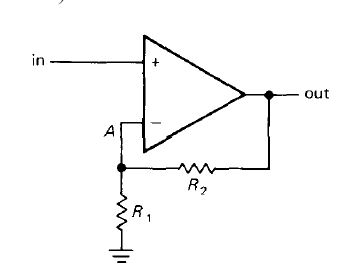
\includegraphics[scale=1]{Op-Amp_Standard}
\caption{Standard configuration of op-amp as a buffer}
\label{fig:op-amp_standard}
\end{figure}

\begin{equation}
gain = 1 + \frac{R_{2}}{R_{1}}
\label{eqn:op-amp_gain}
\end{equation}

\subsubsection{Decoupling Capacitors}
In order to reduce noise on the power supply line to each component, decoupling capacitors were added to each device between the voltage input and ground.
Decoupling capacitors act as low-pass filters, thus removing high frequency voltage differentials.
To ensure no inductance due to the transmission length between the decoupling capacitors and device inputs, the transmission length was minimized \cite{ArtofElectronics}.


\subsection{Printed Circuit Board}
\label{sec:PCB}
In order to combine the system in an efficient manor, it was decided that a printed circuit board (PCB) must be designed to carry the components.
This would make future sensor packages easy to manufacture for additional sensor nodes on the bridge and ensures consistency between packages.
It should be noted that all schematics and circuit board files were created using National Instruments Multisim 13.0 and Ultiboard 13.0 respectfully.
All schematics and board files may be found at \url{https://github.com/mpiannucci/SeniorDesign/tree/master/hardware}.
 
\subsubsection{Requirements for PCB}
Initially the requirements for the PCB were to create a carrier board that would allow for the addition and removal of package components via header sockets.
This would allow for the purchase of many off-the-shelf components that would be able to be installed with minimal effort.
For various reasons, the scope of the PCB was change from being a carrier board to completely integrating all of the components.
This posed difficulties as many of the components utilized in the package were bought as standalone solutions with dedicated PCBs for each component.
As a solution for this, all component that shipped with PCBs had all of their circuitry mimicked on the main PCB.
This holds true for all components except for three; BeagleBone Black, Trimble Copernicus II GPS receiver and the XBee Pro S3B wireless receiver.
It was decided that it was more appropriate to create sockets for each of these components to plug into for specific reasons.
Although the board files for the BeagleBone Black are readily available to download, it was deemed unnecessary to recreate the board.
For the Trimble Copernicus II GPS receiver, it was decided that because of the sensitivity in the design of the antenna circuit that it would be best to use the off-the-shelf board.
The board purchased has the antenna circuit integrated with impedance matched SMA connector for the antenna.
Due to unforeseen issues with interfacing the XBee Pro S3B wireless receivers, the receiver was not incorporated in the initial version of the system design.
Section \ref{sec:XBeeFuture} discusses the future work to be done with the XBee Pro S3B receivers.

\subsubsection{Progress on Printed Circuit Board}
All component footprints for components in the sensor package were created in Multisim 13.0 and Ultiboard 13.0.
The library of components may be found at \url{https://github.com/mpiannucci/SeniorDesign.git} under \verb|./hardware/UsrComp_S_SHMComps.usr|.
A basic board was laid out, however trace routing was not completed due to unresolved net issues.
Although the board design was not finished, a comprehensive schematic was created and will prove useful for future development of the board.
The schematics may be found in Appendix \ref{app:Schematic}.
	\section{Software Design}
		%\section{Software Design}
The software design controls the timing and data collection for the
package. The software structure is simple, yet crucial. In order to
keep the data collected by the package relevant, the software
logic and timing needed to be in order. \\

The first state in the software design is the initialization state.
Here, the analog to digital converter was initialized through I2C
communication. The handle of the analog to digital communication
object was saved for later use in the next state. Once the
initialization state was finished, the application proceeded
to the sampling state.\\

In this application, 200 Hz was decided to be the target sampling
rate. The program waited for an interrupt then the system time 
has reached a user-defined time. This is important because every 
sensor package waited for the same time and they sampled  
at the same instant (accurate to a millisecond). When the signal was received, 
the application proceeded to collect data from the peripheral sensors. For
each sample during the sampling duration, data was collected
from the ADC via I2C. The data structure was appended over the sampling entire
sampling period and passed as a return from the state.
Once the sampling duration was over, the data logging
state was begun. \\

The data logging state received the data structure created in the
previous sampling state. This data was then sorted and written to a
standard comma delimited text file. The file stream was closed
once all of the data had been written and the program finishes. A
simple block diagram of this flow can be seen in Figure
\ref{fig:PRO_SoftFlow}.

\begin{figure}[H]
\centering
\includegraphics[width = 4in]{"Software flow"}
\caption{\textit{Software flow of the sensor package}}
\label{fig:PRO_SoftFlow}
\end{figure}
	\section{Package Power}
		\subsection{Power Budget}
		\subsection{Energy Scavenging Potential}
			\subsubsection{Wind Potential}
			\subsubsection{Solar Potential}
		\subsection{Battery Selection}
		
\chapter{Data Collection}
\label{ch:DataCollection}
	\section{Phase One Data Collection}
		\subsection{6g Tri-Axial Accelerometer Data}
			\chapter{Data Collection}

\subsection{Phase One Data Collection}

\subsubsectin{6g Tri-Axial Accelerometer Data }

\indent Vibration data for the L beam were collected with a microphone, piezoelectric strip, 3g accelerometer to computer, and 6g accelerometer from the sensor package.The only results discussed in this section are those collected from the 6g accelerometer, other results can be viewed in Appendix ()\\
\indent Vibration frequencies of the angle beam were captured by mounting the 6g accelerometer to the beam and striking the beam. The 3” x 3” aluminum angle beam of 3/16 thickness was placed open end down with right angle pointing upward during striking. Configurations varied for supports, strike locations, and accelerometer placement locations. \\
\indent The accelerometer was used to gather vibration data at four different locations. These were at a distance of L/2, L/3, L/4 and L/5 from the angle support, where L is 240” (the length of the supported section of beam).\\
\indent For each accelerometer position, the beam was struck at distance L/8, L/10 and L/16 from the angle support. During the tests using the accelerometers, the beam was struck gently as to minimize or prevent clipping by exceeding accelerometer range of measurement.\\

	\section{Phase Two Data Collection}
		\subsection{6g Tri-Axial Accelerometer Data}
		\subsection{Cell Phone Accelerometer}
		\subsection{Battery Discharge Curve}
		\subsection{Experimental Observed Efficiency}
		
\chapter{Data Analysis}
\label{ch:DataAnalysis}
	\section{Phase One Data Analysis}
		\subsection{Comparison of Preliminary Abaqus Model and Preliminary Data}
			%\chapter{Data Analysis}
%
%\section{Phase One Data Analysis}
%
%\subsection{Comparison of Preliminary Abaqus Model and Preliminary Data }

\indent The results of the best experimental data for the 6g
 accelerometer on the angle beam are shown in Table
  \ref{tab:Results_Comp}.\\
\begin{table}
\begin{center}
    \begin{tabular}{|l| p{3.5cm}| p{3cm}| p{3cm}| p{3cm}|}
    \hline
    \textbf{Mode} & \textbf{Analytical Values} & \textbf{Values for the generalized profile} & \textbf{Values for the Input profile} & \textbf{Experimental} \\\hline
    1    & 3.1 Hz            & 3.1 Hz                             & 3.1 Hz                       & 3.2 Hz       \\\hline
    2    & 12.4 Hz           & 12.5 Hz                            & 12.4 Hz                      & 12.5 Hz      \\\hline
    3    & 27.9 Hz           & 27.8 Hz                            & 27.8 Hz                      & 27.6 Hz      \\\hline
    4    & 49.6 Hz           & 48.8 Hz                            & 48.6 Hz                      & 48.4 Hz      \\\hline
    5    & 77.5 Hz           & 74.5 Hz                            &                             & 78.5 Hz      \\\hline
    \end{tabular}
    \caption{\textit{Comparison between analytical, model and experimental results}}
    \label{tab:Results_Comp}
\end{center}
\end{table}
\begin{table}
\begin{center}
    \begin{tabular}{|l|l|l|l|}
    \hline
    Mode & Analytical Frequencies [Hz] & Experimental Frequencies [Hz] & Percent Difference \\
    \hline
    1    & 3.1                         & 3.2                           & 3.1                \\
    2    & 12.4                        & 12.5                          & 0.80               \\
    3    & 27.9                        & 27.6                          & 1.1                \\
    4    & 49.6                        & 48.4                          & 2.5                \\
    5    & 77.5                        & 78.5                          & 1.3                \\
    \hline
    \end{tabular}
    \caption{\textit{Comparison between analytical and experimental results}}
    \label{tab:ExperimentalvsAnalytical}
\end{center}
\end{table}
A direct comparison between the experimental values and the frequencies may be found in Table \ref{tab:ExperimentalvsAnalytical}.
As the experimental data and the analytical values are very similar the 6g accelerometer can be considered to be taking viable, accurate data.
The first test was done using a piezoelectric strip to detect vibration. The second series of tests was done with a 3g accelerometer (anything above acceleration of 3g is clipped). The third series was done with a 6g accelerometer.

	\section{Phase Two Data Analysis}
		\subsection{Comparison of Developed Abaqus Model with Literature}
			%\subsection{Phase Two Data Analysis}
%
%\subsubsection{Comparison of Developed Abaqus Model with Literature}


In verifying the results of the model produced in Abaqus experimental data taken on the Claiborn Pell Bridge that were published in the Journal of the
Structural Division.
Upon completion in 1969 a study involving seven seismometers estimated the first 20 modes, 11 normal modal response shapes, and 20
critical damping locations.
Traffic, wind, and other environmental factors loading was measured by seismometers. The direct power spectral density by
way of the Ambient Vibrations Survey method was found of each recorded motion, estimates of the natural frequencies were produced.
An Ambient Vibration Survey (ASV) was performed on the bridge on August 20-22, 1969.
During experimentation, approximately 8,000 vehicles passed over the bridge each day
and winds were moderate. Seven seismometers were arranges in five different orientations to properly capture the modal shapes.
20 natural frequencies, 11 normal mode shapes, and 20 critical damping estimates are presented.
The First 20 modes of vibration ranged from 0.155-0.993 Hz,
modal shapes for the first 5 symmetric vertical modes can be seen in \ref{fig:Paul_Modes1-5}\\

%\begin{figure}[h]
%\centering
%\includegraphics[width=\linewidth]{Paul_Modes1-5}
%\caption{The modal response for the first five modes of the Claiborn Pell Bridge.}
%\label{fig:Paul_Modes1-5}
%\end{figure}

In table \ref{tab:FirstFive} the first five modal frequencies produced by the Abaqus model and that indicated by the Journal article. 
The fatigue that has occurred to the bridge since 1969 will account for some of the discrepancies between the frequencies as the bridge will now vibrate differently 
The maximum relative difference is \textbf{\textit{PLACEHOLDER}}, which shows that the frequencies calculated by Abaqus compare well with the measured and analyzed values. 
The main dynamic response properties of the Claiborn Pell Bridge are included in the FEM, which concur with the journal article. 
It is efficient to study the modal properties of the bridge using the FEM.


\begin{table}
\begin{tabular}{|l|l|l|l|}
\hline
Mode &  Journal Article Frequencies [Hz] & Abaqus Model Frequencies [Hz]  & Percent Difference   \\
\hline
1    & 0.16                          & 0.135                              & 15.62\%                \\
2    & 0.42                          & 0.151                           	  & 64.04\%                \\
3    & 0.52                          & 0.161                              & 69.03\%              \\
4    & 0.64                          & 0.224                              & 65.00\%            \\
5    & 0.71                          & 0.259                              & 62.51\%          \\
\hline
\end{tabular}
\caption{\textit{First five modes comparison for Abaqus and Journal Article}}
\label{tab:FirstFive}
\end{table}

As the frequencies are comparable, modal shape concurrence can be looked at. The following is the modal response of the bridge as indicated by Abaqus in \ref{fig:ABAQUS_Chris}. 

\begin{figure}[h]
\centering
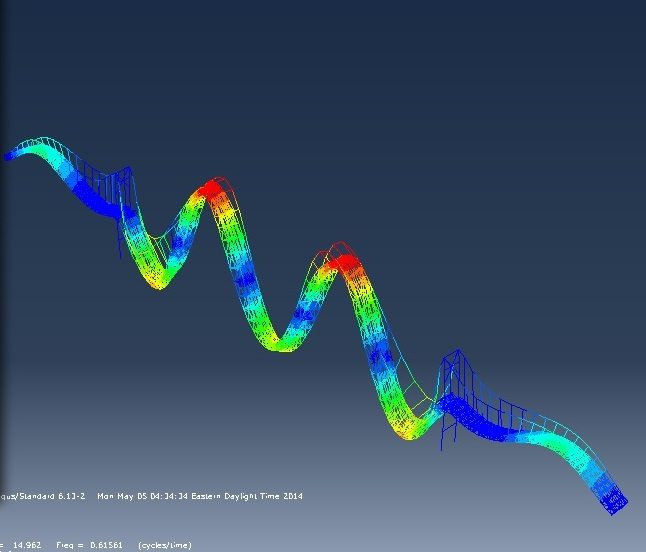
\includegraphics[scale=1]{5th_symm_vert_no_weight}
\caption{\textit{Modal Response of Abaqus Model}}
\label{fig:ABAQUS_Chris}
\end{figure}

		\subsection{Comparison of Developed Abaqus Model with Developed Abaqus Model}	
		
\chapter{Future Development}
\label{ch:FutureDevelopment}
	\section{Instrumentation}
		\subsection{Integration of Strain Gauge}
			\subsubsection{Integration of Strain Gauge}

\indent Figure \ref{fig:OmegaSoldered} is one of the 3-element rosette strain gauges with pre-soldered ribbon leads. Purchased from omega engineering with
model number SGD-6/120RYT23. These strain gauges were necessary after realizing the difficulty of soldering leads to the original set of strain gauges. The
pre-soldered ribbon leads on the second set of strain gauges also proved to be unsuccessful during experimentation. This was because the leads would not
stay secured to the attaching clips while tests were being run. Even with the persistent attempts to get the strain gauges connected and working
correctly, the data received was still very inaccurate. One possible contributing factor to this may have be the lack of precision when applying the
strain gauge to the exact location on the beam. However, one definite factor that contributed to the inaccurate data from the strain gauges was the
type of strain gauge that was used. A strain gauge with a different gauge factor and a higher resistance would have been more favorable. The higher
the resistance of a strain gauge, the higher the sensitivity. The original sets of strain gauges had a resistance of 120 $\Omega$, but to precisely
measure strain on a beam the resistance must be much higher, 350 $\Omega$ or more. The costs for a pack of 6 similar strain gauges with a resistance of
350 $\Omega$ from omega engineering is one hundred dollars. Another factor that halted the efforts to apply the strain gauge was that they required
another ADC output. It is possible to make more outputs, however this also demands that the time synchronization is even more accurate.
Nevertheless, higher resistant strain gauges would be better for sensor packages for future developments. \\

\begin{figure}[h]
\centering
\includegraphics[width=0.3\textwidth]{Strain_Gauge_with_Leads.png}
\caption{Omega 3-Element Rosette with pre-soldered leads.}
\label{fig:OmegaSoldered}
\end{figure}
		\subsection{Wireless Transmission}
			\label{sec:XBeeFuture}
		\subsection{GPS Time Synchronization}
		\subsection{Package Assembly}
			\subsubsection{Fabrication of Circuit Board}
			\subsubsection{Battery Integration}
			\subsubsection{Power Management}
			\subsubsection{Package Enclosure}
				\paragraph{Casing}

When the components are tested and fully operational in laboratory conditions, they will need to be packaged into the casing.  The following
characteristics need to be considered when determining which case is best suited for this application:

\begin{itemize}
\item {Quality} 
\item {Size/Orientation}
\item {Heat Dissipation} 
\item {Cost} 
\item {External Connectors}
\end{itemize}


When the package is mounted onto the Newport Bridge, it will be exposed to harsh weather conditions: wind, precipitation, extreme temperatures,
etceteras.  Therefore, it is essential to utilize a case that can withstand these conditions.  O-rings are necessary to prevent water from leaking into
the case through the seal of the lid.  This water can easily damage the electrical components within the package.  The case will also have to be able to
withstand possible extreme temperatures.  If the case cannot withstand the possible cold temperatures it will be exposed to without cracking, water can
leak into the package and destroy the equipment.  High temperatures can cause the case to melt/deform which may possibly affect the retrieved data.  

It will be important to choose a case that not only large enough that can house all of the equipment but also fits the equipment in a manner that it can
be neatly organized and arranged.  This allows for a quicker and more efficient package assembly.  This also allows for a quicker examination of the
set-up in case an error occurs.  To account for this, the orientation of the case is important.  For example, a top-loading bucket (such as the Pelican
1430 seen below) would not be practical because it would be very difficult to access the components once the package is assembled and mounted.   



Electrical devices are only operational within a specific temperature range where if the maximum or minimum temperatures are exceeded, the component may
not fully function or even fail completely.  To determine if the SHM system will fail due to extreme temperatures, the temperature inside the case must
be calculated.  The enclosed volume has two major sources of temperature flux: the external temperature and the work done by the system.  The first step
will be to calculate the heat transferred from the electrical components using the equation:

\begin{equation}
q(eq) = P(eq)*K_1*K_2
\end{equation}

where $q(eq)$ is the heat transferred from electrical equipment in Watts (W), $P(eq)$ is the electrical power consumption (W), $K_1$ is the load
coefficient, and $K_2$ is the running time coefficient.  This value will then be inserted into the 1-D heat transfer equation:

\begin{equation}
q=k*A*\frac{\Delta T}{dx}
\end{equation}

where $q$ is the heat due to the electrical components, $k$ is the thermal conductivity of the material, $A$ is the area of which heat is being transfered
through, $\Delta T$ is the change in temperature, and $dx$ is the thickness of material. This equation will need to be computed for the heat transfer
through each of the casing walls, as well as the corners of the case, then averaged using the equation: 

$$q_t = sqrt((q_x)^2+(q_y)^2+(q_z)^2+(q_c)^2)$$

where $q_c$ is the heat transfer through the corners of the case. The resulting value will then be used with the maximum expected temperatures based on
temperature history data, such as that provided by NOAA, to determine the maximum temperature at which the system will still operate. If the resulting
temperature is higher than the lowest maximum operating temperature out of all the components, the system may fail, and that case may not be the best
option. That same principal can be applied to when the system is not generating any heat with respect to the minimum expected external temperature and
highest minimum operational temperature of the components. Ideally, once the package is fully modeled, the heat transfer equation can be more
thoroughly and accurately calculated by accounting for the spatial orientation between the components and the interior walls of the case. However,
if the components are mounted in place via foam cutouts, the heat dissipation between the components and the foam must first be calculated, and then
the heat transfer between the foam and the interior walls will then be calculated.

\paragraph{External Connectors} 
Several external connectors will need to be installed on the case walls for the full functionality of the SHM system. These ports need to be waterproof
with tight seals to prevent water from entering the case or external connections. The waterproof connections will require secure mating mechanisms, such
as locking and screwing mechanisms shown in Figure~\ref{fig:BowChicaWowWow}, to ensure that that the male ends will not become unplugged thus allowing
water to enter the connection and damage it. Each connector will also require a bulkhead cap to cover and protect against water damage if the
connector is not in use. These external connections are going to be implemented for a variety of sub-systems within the SHM package: energy
scavenging devices, BeagleBone Black, strain gauge, GPS, and XBee.
\begin{figure}[h]
\centering
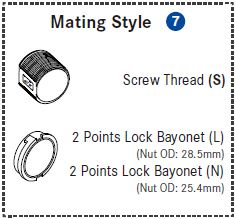
\includegraphics[width=0.3\textwidth]{Wiley_MatingStyle.JPG}
\caption{\label{fig:BowChicaWowWow} Example Mating Mechanisms}
\end{figure}

Power connectors will be used to connect the wind turbine and solar panels to the package. These connectors must be rated for a high enough current to
match the power source. For example, since the wind turbine is rated up to 27A, the power connector should have a current rating that is similar enough
that there will not be damage done to the port due to the excess current. Each power connection will have a female port installed on the side of the
case and a corresponding male jack will need to be installed at the end of the power input. If multiple solar panels are utilized, either the power
inputs need to be put into parallel in one wire to input all the energy through one connection or a connector needs to be installed for as many panels
are used. 

A USB 2.0A port will be installed to access the BBB without having to open the package via a flash drive. This type of USB port was chosen to match the
same type of connection specified from the BBB data sheet. The connector gender of this port needs to be female to plug a USB chord to access the BBB,
such as the one seen in Figure \ref{fig:USB}. 
\begin{figure}[h]
\centering
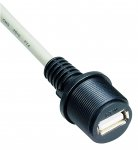
\includegraphics[width=0.3\textwidth]{Wiley_USB2Aport.JPG}
\caption{\label{fig:USB} USB 2.0A External Connector (LTWUA-20AMFM-SL7A) from Ampehnol LTW}
\end{figure}

There are a few different types of connectors that can be used to attach the leads of the strain gauge to the package. Unlike the rest of the
connections, the strain gauge leads do not require a certain type of connection terminal. One option is to attach the leads to either a category 5 (CAT
5) or CAT5e shielded Ethernet cable and install an external connection for such a cable as seen in Figure~\ref{fig:CAT5}. Category type cables are
designed for high signal integrity to achieve performance standards set by organizations (such as IEEE) (citation). \todo{this citation was exported
form Google as a .BibTex file.}. This type of cable will ensure that the signals are relayed to the ADC reliably. A shielded cable is desired to
ensure that the sensitive signal being sent from the strain gauge to the ADC does not get disturbed by noise. 
\begin{figure}[h]
\centering
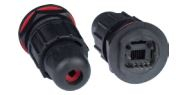
\includegraphics[width=0.3\textwidth]{Wiley_CAT5EthernetConnection.JPG}
\caption{\label{fig:CAT5} Shielded Ethernet External Connector (RJ45-5EWTP-QR-PCB) from Video Production Inc}
\end{figure}

An alternative method is through the use of waterproof cable glands (see Figure~\ref{fig:Cable Gland}. The leads would be attached to a cable, preferably
shielded, and fed through the gland which would then be sealed. The proper gland must be matched up to the outer diameter of the cable otherwise the
gland will not be water tight. These are advantageous because not only do individual cable glands work with a range of cable thicknesses, but different
gland diameter ranges can be found. 
\begin{figure}[ht]
\centering
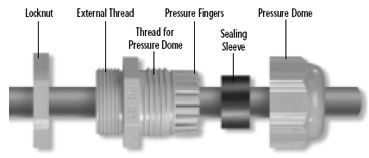
\includegraphics[width=0.7\textwidth]{Wiley_CableGland.JPG}
\caption{\label{fig:Cable Gland} Cable Gland (CB-GD-5000045) from AA Power Corp}
\end{figure}


The GPS antenna attaches to the GPS via the use of a coaxial MCX connection. Two viable options for connecting the antenna are to implement a waterproof
MCX connector or a cable gland. Implementing a waterproof MCX connector on the package may be difficult because MCX connectors are very small as evident
by Figure \ref{fig:MCX}. If one of these connectors is able to implemented, it will be essential to choose the proper impedance level of the
connector. The other option is to implement a cable gland, such as the alternative option for the strain gauge above in Figure~\ref{fig:Cable Gland},
to run a wire through the case wall between the antenna and the GPS. The antenna would then need to be fastened to the outside of the case or another
substrate to prevent it from freely swinging around. 
\begin{figure}[ht]
\centering
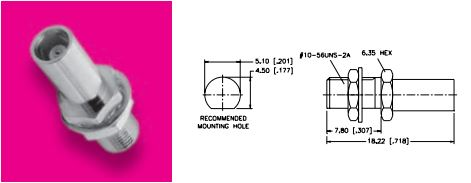
\includegraphics[width=0.7\textwidth]{Wiley_MCX.JPG}
\caption{\label{fig:MCX} MCX Jack-to-Jack Adapter (252171) from Aamphenol Connex with Size Reference}
\end{figure}


The final component that requires and external connector is the XBee.The XBee antenna attaches to the device itself via the use of an SMA connection. A
waterproof coaxial connector, like the one shown in Figure~\ref{fig:SMA}, can be implemented as the external connector as well as a cable gland. 
Similarly to the MCX connector, the SMA connector is also small which may make utilizing one of these difficult. However, if a cable gland is used, the
antenna may need to be mounted to the case or other substrate to prevent it from freely swinging around as is the case with the GPS.
\begin{figure}[ht]
\centering
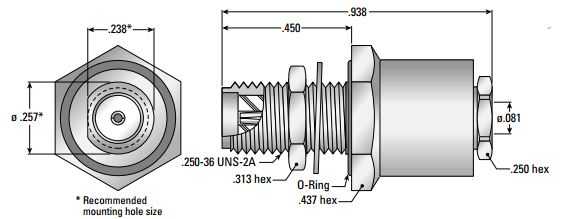
\includegraphics[width=0.7\textwidth]{Wiley_SMAconnector.JPG}
\caption{\label{fig:SMA} Waterproof SMA Bulkhead Connector (9153-7553-002) from Applied Engineering Products with Size Reference}
\end{figure}



\paragraph {Case Selection} Attempts were made to try to obtain the actual thermal conductivity coefficients for different cases, but unfortunately proper
data was never able to be retrieved due to lack of information from retailers. Since the general material of the considered cases is known, an
estimation of the thermal conductivity coefficient was made because studies have been performed to determine $k$ values for different materials. 
However, continued efforts to obtain this information may supply data to more accurately calculate the heat transfer through the casing walls. The
thickness of each case will need to be considered for two reasons. The first reason is that the thickness of the case affects heat transfer. Thicker
cases will allow for less heat transfer through the casing walls. The other is that the thickness of the casing wall affects whether or not certain
external connectors can be implemented. If the case is too thick, many MCX and SMA connectors may not be able to be installed because the case may
be thicker than the connector is long. When comparing costs, it should be later noted of any accessories, whether they are necessary or
convenient, that can and will be purchased. For example, the Ultra-case 613 by UW Kinetics charges another \$6.99 for the required O-ring to
water proof an already expensive case, so this may not be the most suitable case for this application. For a look at the a comparison of nominal
characteristics of the cases that were considered, see \ref{sec:Appendix Case Comparison}.

\paragraph{Assembly Layout}


When the package is ready to be assembled, the interior layout of the components needs to be determined. A few factors will need to be considered. 
The first is the location of external connectors. As stated above, the thickness of the case will affect what type of connectors may need to used. 
An example of this is shown in Figure \ref{fig:Assembly} which is a potential 2-D assembly layout using a Pelican 1400 model case. If an SMA
connector is used instead of a cable gland, it would need to be installed on the shorter wall since the case does not have a uniform thickness and
that wall is the only one thin enough out of the two to install such a connector. It would not make to sense to install the connectors through
the lid either because opening the case may place too much tension on the wires causing damage. 

\begin{figure}[h]
\centering
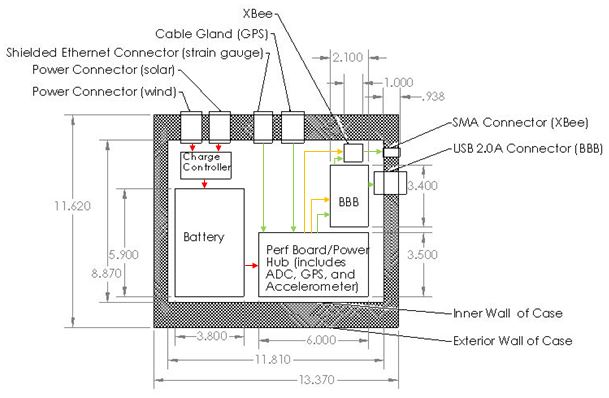
\includegraphics[width=1\textwidth]{Wiley_2DAssemblyLayout.jpg}
\caption{\label{fig:Assembly} Potential Layout of a Pelican 1400 Model Case}
\end{figure}

It will also be important to orient the breadboard in a manner that the accelerometer measures data in the intended direction as if it was mounted. 
Otherwise, it will need to be understood that the data measured on each axis during lab trials will not be measured along the same axes in the field and
will need to be accounted for while analyzing the data. 

\paragraph{Package Location}

\indent Figure \ref{fig:PackageLocation} is an Abaqus visualization of the Newport Bridge with the proposed location for the sensor package to be mounted.
As shown in the figure, the center of the bridge is the best location for the sensor package. This is because the greatest amplitude of displacement will
occur during the first mode of vibration at the middle of the bridge. Mounting the sensor package to the bridge must be done without damaging the
structure in any way. The sensor package must also be capable of being moved easily. Most importantly, the package must be secured without any of its
own motion so that the sensors can recognize the movement of the bridge and not the movement of the package itself. 

The most economical way of securing the sensor package to the bridge is to use powerful magnets. Neodymium Magnets are strong magnets that work well in
all environments and resist demagnetization. One negative aspect of magnets is that they can be prone to corrosion if a protective coating is not
properly applied. There is also a concern that the magnetic field can disrupt the electronics within the case. However, these issues can be prevented if
the correct precautions are taken. These magnets come in many shapes and sizes, as shown in Figure \ref{fig:Mounting Magnet}, and can be purchased with
pre-fabricated holes for screws to attach the magnets to the exterior of the case. The magnets in figure \ref{fig:Mounting Magnet} are the MMR-A-XC
model of magnets from KJMagnetics.com. This magnet is hardly larger than a penny, yet it can easily be screwed into the sensor package and has a
holding force of 54.14 pounds. With two of these magnets screwed into the case, the package would be secured to the bridge. If data analysis is
performed to prove the wind speed on the surface of the package to be too much for this pull force, stronger magnets are available. KJMagnetics.com
also has similar magnets but with different pull forces ranging from 26.8 pounds to 260 pounds. These magnets can be used for securing the solar
panels and wind turbine as well. 

\begin{figure}[ht]
\centering
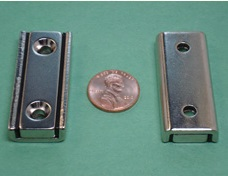
\includegraphics[width=0.3\textwidth]{Neodymium_Mounting_Magnet.jpg}
\caption{Neodymium Mounting Magnet.}
\label{fig:Mounting Magnet}
\end{figure}

Figure \ref{fig:Proposed Package, Panels and Turbine Location} shows a practicable location for the sensor package along with the solar panels above and
the wind turbine hanging just below. The sensor package should be mounted on the outside of one of the major vertical beams at midspan of the bridge. The
solar panels and wind turbine must be mounted close within a reasonable distance to keep the cable length to a minimum. The best place to mount the
solar panels is on top of the upper horizontal beam on the southern side of the bridge. This will allow for the most amount of sun light and the
shortest amount of cable necessary. The best place to mount the wind turbine is on the bottom of the lower horizontal beam on the southern side of the
bridge. This location has plenty of wind because it is above the middle of the Narragansett Bay. By mounting the sensor package, solar panels and
wind turbine below the deck on the southern side of the bridge the package will be capable of producing its own power and accurately measuring the
vibrations of the bridge.


\begin{figure}[ht]
\centering
\includegraphics[width=0.3\textwidth]{Bridge_Full_.png}
\caption{Proposed Package Mounting Location.}
\label{fig:PackageLocation}
\end{figure}


\begin{figure}[ht]
\centering
\includegraphics[width=0.3\textwidth]{Proposed_Package_Location.png}
\caption{Proposed Location for Sensor Package, Wind Turbine and Solar Panels.}
\label{fig:Proposed Package, Panels and Turbine Location}
\end{figure}




\section{Appendix Case Comparison}
\begin{table}[h]
\begin{tabular}{lllllllp{3cm}}
Company   & Case Model   & Length & Width & Height & Weight & Cost   & Thermal Conductivity Coefficient (W/m*$^{\circ}$C) \\
Pelican   & 1300      & 9.17  & 7.00 & 6.12  & 3.09  & \$55.65 & 0.1-0.22                       \\
~      & 1400      & 11.81 & 8.87 & 5.18  & 3.97  & \$81.58 & 0.1-0.22                       \\
~      & 1450      & 14.62 & 10.18 & 6   & 5.51  & \$103.73 & 0.1-0.22                       \\
~      & 1460      & 18.54 & 9.92 & 10.92 & 8.75  & \$180.59 & 0.1-0.22                       \\
Fibox    & PC MH 125 G  & 9.1  & 5.5  & 4.9  & NA   & NA    & 0.19                         \\
~      & PC 2828 18 G  & 10.9  & 10.9 & 7.1  & NA   & NA    & 0.19                         \\
~      & PC 175/150 XHG & 7.1  & 7.1  & 5.9  & NA   & NA    & 0.19                         \\
Nanuk    & 9.4      & 9.4  & 7.4  & 5.5  & 3.3  & \$38.95 & 0.1-0.22                       \\
~      & 915      & 13.8  & 9.3  & 6.2  & 4.4  & \$63.95 & 0.1-0.22                       \\
UW Kinetics & Ultra-case 613 & 13.4  & 8.9  & 5.6  & 4.5  & \$148.99 & 0.2                         \\
\end{tabular}
\end{table}

			\subsubsection{Package Location}
				\section{Package Location}

\indent Figure \ref{fig:PackageLocation} is an Abaqus visualization of the Newport Bridge with the proposed location for the sensor package to be mounted.
As shown in the figure, the center of the bridge is the best location for the sensor package. This is because the greatest amplitude of displacement will
occur during the first mode of vibration at the middle of the bridge. Mounting the sensor package to the bridge must be done without damaging the
structure in any way. The sensor package must also be capable of being moved easily. Most importantly, the package must be secured without any of its
own motion so that the sensors can recognize the movement of the bridge and not the movement of the package itself. 

The most economical way of securing the sensor package to the bridge is to use powerful magnets. Neodymium Magnets are strong magnets that work well in
all environments and resist demagnetization. One negative aspect of magnets is that they can be prone to corrosion if a protective coating is not
properly applied. There is also a concern that the magnetic field can disrupt the electronics within the case. However, these issues can be prevented if
the correct precautions are taken. These magnets come in many shapes and sizes, as shown in Figure \ref{fig:Mounting Magnet}, and can be purchased with
pre-fabricated holes for screws to attach the magnets to the exterior of the case. The magnets in figure \ref{fig:Mounting Magnet} are the MMR-A-XC
model of magnets from KJMagnetics.com. This magnet is hardly larger than a penny, yet it can easily be screwed into the sensor package and has a
holding force of 54.14 pounds. With two of these magnets screwed into the case, the package would be secured to the bridge. If data analysis is
performed to prove the wind speed on the surface of the package to be too much for this pull force, stronger magnets are available. KJMagnetics.com
also has similar magnets but with different pull forces ranging from 26.8 pounds to 260 pounds. These magnets can be used for securing the solar
panels and wind turbine as well. 

\begin{figure}[ht]
\centering
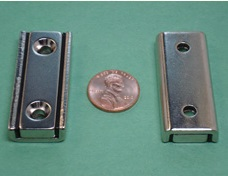
\includegraphics[width=0.3\textwidth]{Neodymium_Mounting_Magnet.jpg}
\caption{Neodymium Mounting Magnet.}
\label{fig:Mounting Magnet}
\end{figure}

Figure \ref{fig:Proposed Package, Panels and Turbine Location} shows a practicable location for the sensor package along with the solar panels above and
the wind turbine hanging just below. The sensor package should be mounted on the outside of one of the major vertical beams at midspan of the bridge. The
solar panels and wind turbine must be mounted close within a reasonable distance to keep the cable length to a minimum. The best place to mount the
solar panels is on top of the upper horizontal beam on the southern side of the bridge. This will allow for the most amount of sun light and the
shortest amount of cable necessary. The best place to mount the wind turbine is on the bottom of the lower horizontal beam on the southern side of the
bridge. This location has plenty of wind because it is above the middle of the Narragansett Bay. By mounting the sensor package, solar panels and
wind turbine below the deck on the southern side of the bridge the package will be capable of producing its own power and accurately measuring the
vibrations of the bridge.


\begin{figure}[ht]
\centering
\includegraphics[width=0.3\textwidth]{Bridge_Full_.png}
\caption{Proposed Package Mounting Location.}
\label{fig:PackageLocation}
\end{figure}


\begin{figure}[ht]
\centering
\includegraphics[width=0.3\textwidth]{Proposed_Package_Location.png}
\caption{Proposed Location for Sensor Package, Wind Turbine and Solar Panels.}
\label{fig:Proposed Package, Panels and Turbine Location}
\end{figure}

	\section{FEM}
		\section {Finite Element Model}

\subsection{Model Improvements}

The Abaqus model produced for this project can be further developed to produce more accurate modal responces to static and dynamic loading. Any improvement to the model will replicate the bridge more closely. The longterm effect of fatigue is immeasurable and will create an unavoidable error. After measuring the current natural frequency of a bridge an origional sitffness matrix can be estimated from the bridge a sfittness matrix can be estimated and inputed to Abaqus, however, evaluation the effects of fatigue on structural integrity is difficult.    
\indent The current model is considered to be one cohesive piece with a uniform stiffness rather than different indivudual sections that are bolted or welded together. In a more precise model, as the 19,0000 element model produced for evaluating the Tsing Ma Bridge in Hong Kong, each piece of the bridge was modeled to reflect the actual material. The steel cables were molded as thousands of steel wires and the road deck was modeled as pavement \cite{Chan}. As steel is primarly used for the entire structure of the Claiborn Bridge the error aquired is relatively small. 
\indent Suspension bridges will deform plastically everywhere accept for the welded regions which should be modled as ridgid pieces. These joints are critical locations in the system as fatigue cracks will develop first. If the welds that are under the most stress can be identified they can be reinforced or monitored more closely \cite{Chan}. Bridge secions that connect at bolts rather than welds have friction at the interface of the two sections. This friction is imporatant when evaluating failure.

\subsection{Dynamic Loading} 

\indent In this evaluation, only static loading was evaluated as dynamic loading is outside the scope of this project. The model of the Tsing Ma Bridge was evaluated for dynamic loading as two mediums of traffic utalize this bridge. The trains and trucks that travel over the bridge require entirely seperste analysis as they present the bridge with entirely different loading signatures.\\
\indent The loading of a train, individual truck in both lanes, and groups of trucks with varying orientation were simulated passing over the bridge. As a single truck will not affect the net dynamic response only the local response must be examined. To minimize computation time only relevant elements were applied a tapering load for less than 2 s and then eliminated from the simulation. Groups of trucks were separated by a 3 s lag time. The variability of traffic was examined and the co-existence of the two types of loading were quantified. A stress cycle was produced for each traffic variation and compiled to identify which element would experience the most intense local stresses. The critical locations of local stress under truck loading are the outmost part of the upper chord and the bottom cross-frame between the rail tracks. Under train loading the critical locations in the deck unit are at the outmost parts of the upper chord and show more stress than the highest local stress under truck loading. Because of this it was determined that an outbound train will produce the most stress in the upper chords along the bridge longitudal direction. This location was chosen to determine fatigue critical locations in the whole bridge \cite{Chan}. 

		
\chapter{Conclusion}
\label{ch:Collection}
	
\chapter{Conclusions}
\indent Over the course of this two phase project a prototype of the sensor package was designed and partially assembled. A finite element model was produced and verified for the Claiborn Pell Bridge.  Development must be done on wireless transmission of data, time-synchronization of data and energy scavenging. It is anticipated that the final sensor package will have a custom PCB designed and fabricated to localize the microprocessor, ADC, accelerometer and GPS to one board.\\
\indent 



\bibliographystyle{plain}
\bibliography{./BIB_Files/WILEY_BIB,./BIB_Files/KIRBY_BIB,./BIB_Files/PAUL_BIB,./BIB_Files/IANNUCCI_BIB}

\appendix

\chapter{Sensor Package Schematics}
\label{app:Schematic}
\section{LM317 Adjustable Voltage Regulators}
\begin{figure}[H]
\centering
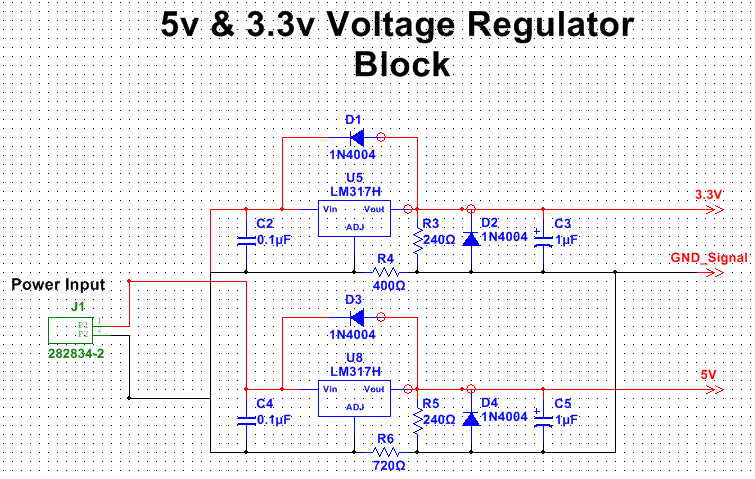
\includegraphics[width=\textwidth,height=\textheight,keepaspectratio]{./KIRBY_Images/Multisim_VoltageRegulation}
\caption{Schematic of 5V and 3.3V voltage regulator circuit}
\label{fig:Schematic_VoltageReg}
\end{figure}

\section{BeagleBone Black}
\begin{figure}[H]
\centering
\includegraphics[width=0.9\textwidth,height=0.9\textheight,keepaspectratio]{./KIRBY_Images/Multisim_BBB}
\caption{Schematic of BeagleBone Black}
\label{fig:Schematic_BBB}
\end{figure}

\section{ADS1113 Analog-Digital Converter}
\begin{figure}[H]
\centering
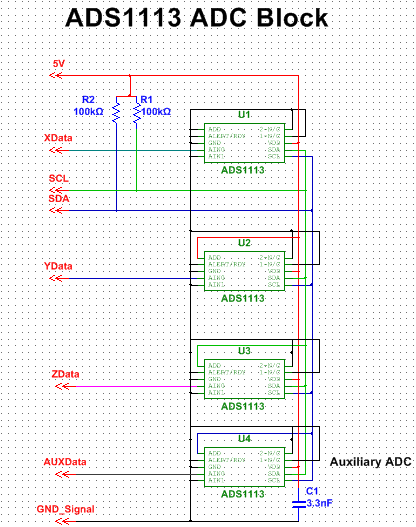
\includegraphics[width=0.9\textwidth,height=0.9\textheight,keepaspectratio]{./KIRBY_Images/Multisim_4ADC}
\caption{Schematic of four ADS1113 ADC units in parallel}
\label{fig:Schematic_ADS1113}
\end{figure}


\section{MMA7361 Accelerometer}
\begin{figure}[H]
\centering
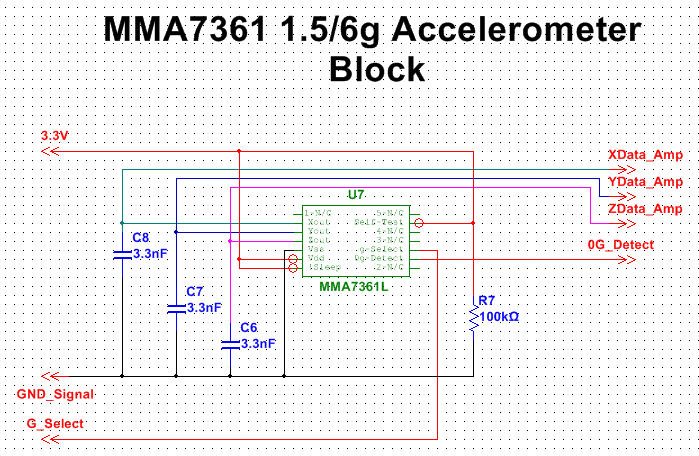
\includegraphics[width=\textwidth,height=\textheight,keepaspectratio]{./KIRBY_Images/Multisim_MMA7361}
\caption{Schematic of MMA7361 $\pm 1.5g/ \pm 6g$ Tri-Axial Accelerometer}
\label{fig:Schematic_MMA7361}
\end{figure}

\section{Trimble Copernicus II GPS Receiver}
\begin{figure}[H]
\centering
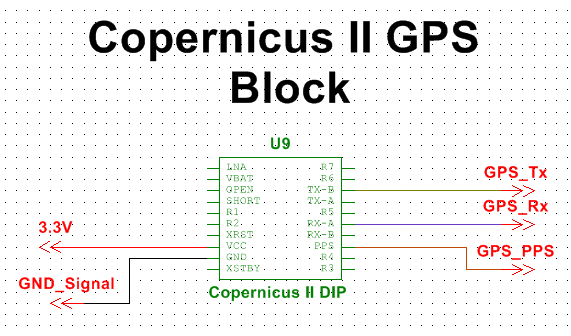
\includegraphics[width=\textwidth,height=\textheight,keepaspectratio]{./KIRBY_Images/Multisim_GPS}
\caption{Schematic of Copernicus II GPS Receiver}
\label{fig:Schematic_Copernicus}
\end{figure}

\chapter{Enclosure Options}
\label{app:CaseOptions}
\begin{landscape}

\begin{table}[c]
\centering
\begin{tabular}{|c|l*{5}{|c}|p{2.5cm}|}
\hline
\multicolumn{8}{|c|}{\textbf{Enclosure Options}}\\
\hline
Company   & Case Model   & Length & Width & Height & Weight & Cost   & Thermal Conductivity Coefficient (W/m*$^{\circ}$C) \\
\hline
Pelican   & 1300      & 9.17  & 7.00 & 6.12  & 3.09  & \$55.65 & 0.1-0.22                       \\
~      & 1400      & 11.81 & 8.87 & 5.18  & 3.97  & \$81.58 & 0.1-0.22                       \\
~      & 1450      & 14.62 & 10.18 & 6   & 5.51  & \$103.73 & 0.1-0.22                       \\
~      & 1460      & 18.54 & 9.92 & 10.92 & 8.75  & \$180.59 & 0.1-0.22                       \\
Fibox    & PC MH 125 G  & 9.1  & 5.5  & 4.9  & NA   & NA    & 0.19                         \\
~      & PC 2828 18 G  & 10.9  & 10.9 & 7.1  & NA   & NA    & 0.19                         \\
~      & PC 175/150 XHG & 7.1  & 7.1  & 5.9  & NA   & NA    & 0.19                         \\
Nanuk    & 9.4      & 9.4  & 7.4  & 5.5  & 3.3  & \$38.95 & 0.1-0.22                       \\
~      & 915      & 13.8  & 9.3  & 6.2  & 4.4  & \$63.95 & 0.1-0.22                       \\
UW Kinetics & Ultra-case 613 & 13.4  & 8.9  & 5.6  & 4.5  & \$148.99 & 0.2                         \\
\hline
\end{tabular}
\caption{Brief summary of enclosure options considered for the sensor package}
\end{table}
\end{landscape}

\chapter{Battery Log}
\label{app:batterylog}
\section{Battery Log}
\label{app:BatteryLog}
%\begin{table}[h]
\centering
\begin{longtable}{|l|l|l|p{2.5cm}|}
\hline
Filename   & 20140421T162625                &          &                                                                               \\
Battery    & 1-3                            &          &                                                                               \\
V initial  & 13.21 V                        &          & Test on new battery 1-3 with car light                                        \\
load       & Sylvania 3157                  &          &                                                                               \\
           & 26.88 W                        & 4.24 $\Omega$   &                                                                               \\
           & 12V                            &          &                                                                               \\
           & 2.1 A                          &          &                                                                               \\
           &                                &          &                                                                               \\
cut out    & 9 V                            & 10:19:39 &                                                                               \\
V open cir & 10.881 V                       &          &                                                                               \\
           &                                &          &                                                                               \\
\hline
Filename   & 20140422T113901                &          &                                                                               \\
Battery    & 1-3                            &          &                                                                               \\
V open cir & 10.881 V                       &          & Log  of open circuit voltage from previous test                               \\
           &                                &          &                                                                               \\
Filename   & 20140422T133734                &          &                                                                               \\
Battery    & 1-3                            &          &                                                                               \\
V initial  &                                &          & After fully discharged battery had rested for 2 hours it was discharged again \\
load       & Sylvania 3157                  & 4.24 $\Omega$   &                                                                               \\
           & 26.88 W                        &          &                                                                               \\
           & 12V                            &          &                                                                               \\
           & 2.1 A                          &          &                                                                               \\
cut out    & 9 V                            &          &                                                                               \\
V open cir & 10.881 V                       &          &                                                                               \\
           &                                &          &                                                                               \\
\hline
Filename   & 20140422T141819                &          &                                                                               \\
Battery    & 3-1                            &          &                                                                               \\
V initial  & 13.20 V                        &          & Part 1 of initial test on battery 3-1                                         \\
load       & 2 x 100Ω resistors in parallel &          &                                                                               \\
           & 49.648 Ω observed              &          &                                                                               \\
           &                                &          &                                                                               \\
\hline
Filename   & 20140423T104026                &          &                                                                               \\
Battery    & 3-1                            &          &                                                                               \\
V initial  & 13.20 V                        &          & Part 2 of initial test on battery 3-1                                         \\
load       & 2 x 100$\Omega$ resistors in parallel &          &                                                                               \\
           & 49.648 $\Omega$ observed              &          &                                                                               \\
cut out    & 8.962 V                        & 20:22:12 &                                                                               \\
V open cir & 10.96 V                        &          &           \\
\hline       
                                                   
\end{longtable}
%\caption{Captions!~}
%\end{table}
 

\end{document}
